\chapter{HASIL DAN PEMBAHASAN}

\section{Hasil Rancangan Sistem Identifikasi Kendaraan Pada Pemarkiran Dengan Pengenalan Citra Dan Pembacaan RFID}

\subsection{Hasil Perancangan Perangkat Keras}
\begin{figure} [H]
    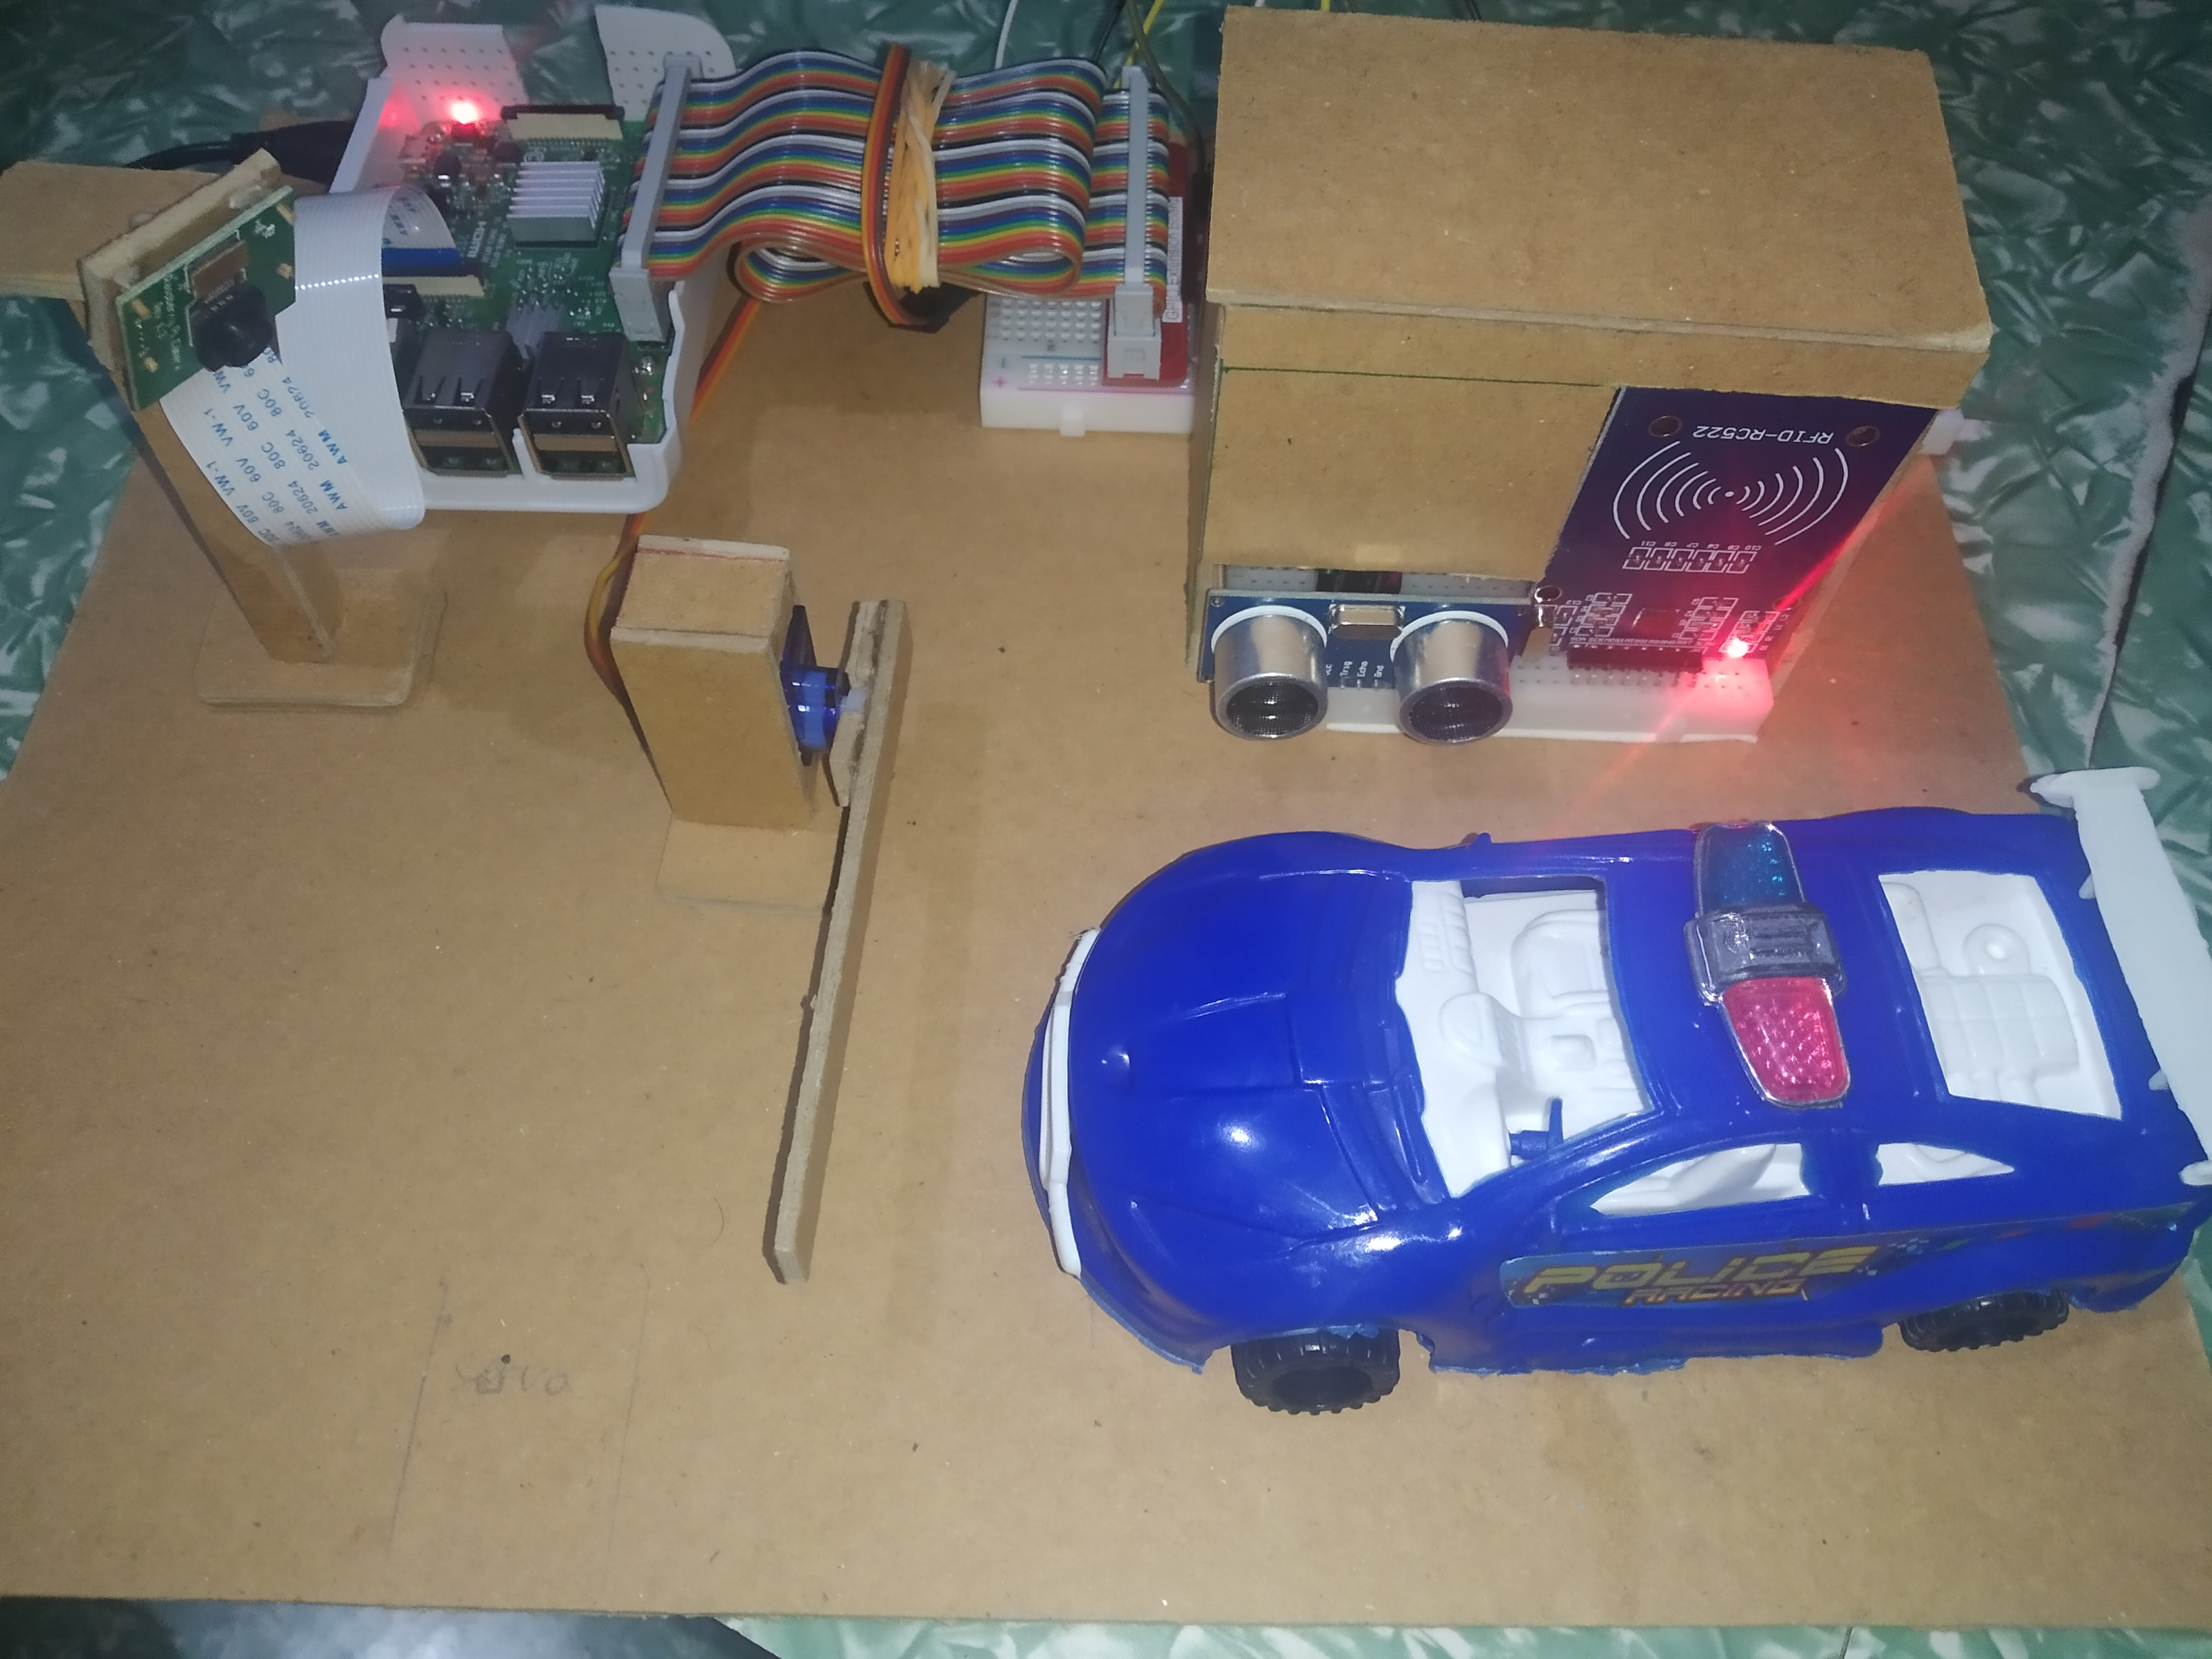
\includegraphics[height=7cm, width=0.5\textwidth, center]{images/alat-full-mobil.jpg}
    \caption{Hasil Rancangan dan Pemasangan Alat}
    \label{fig:alatfullmobil}
\end{figure}

\begin{figure} [H]
    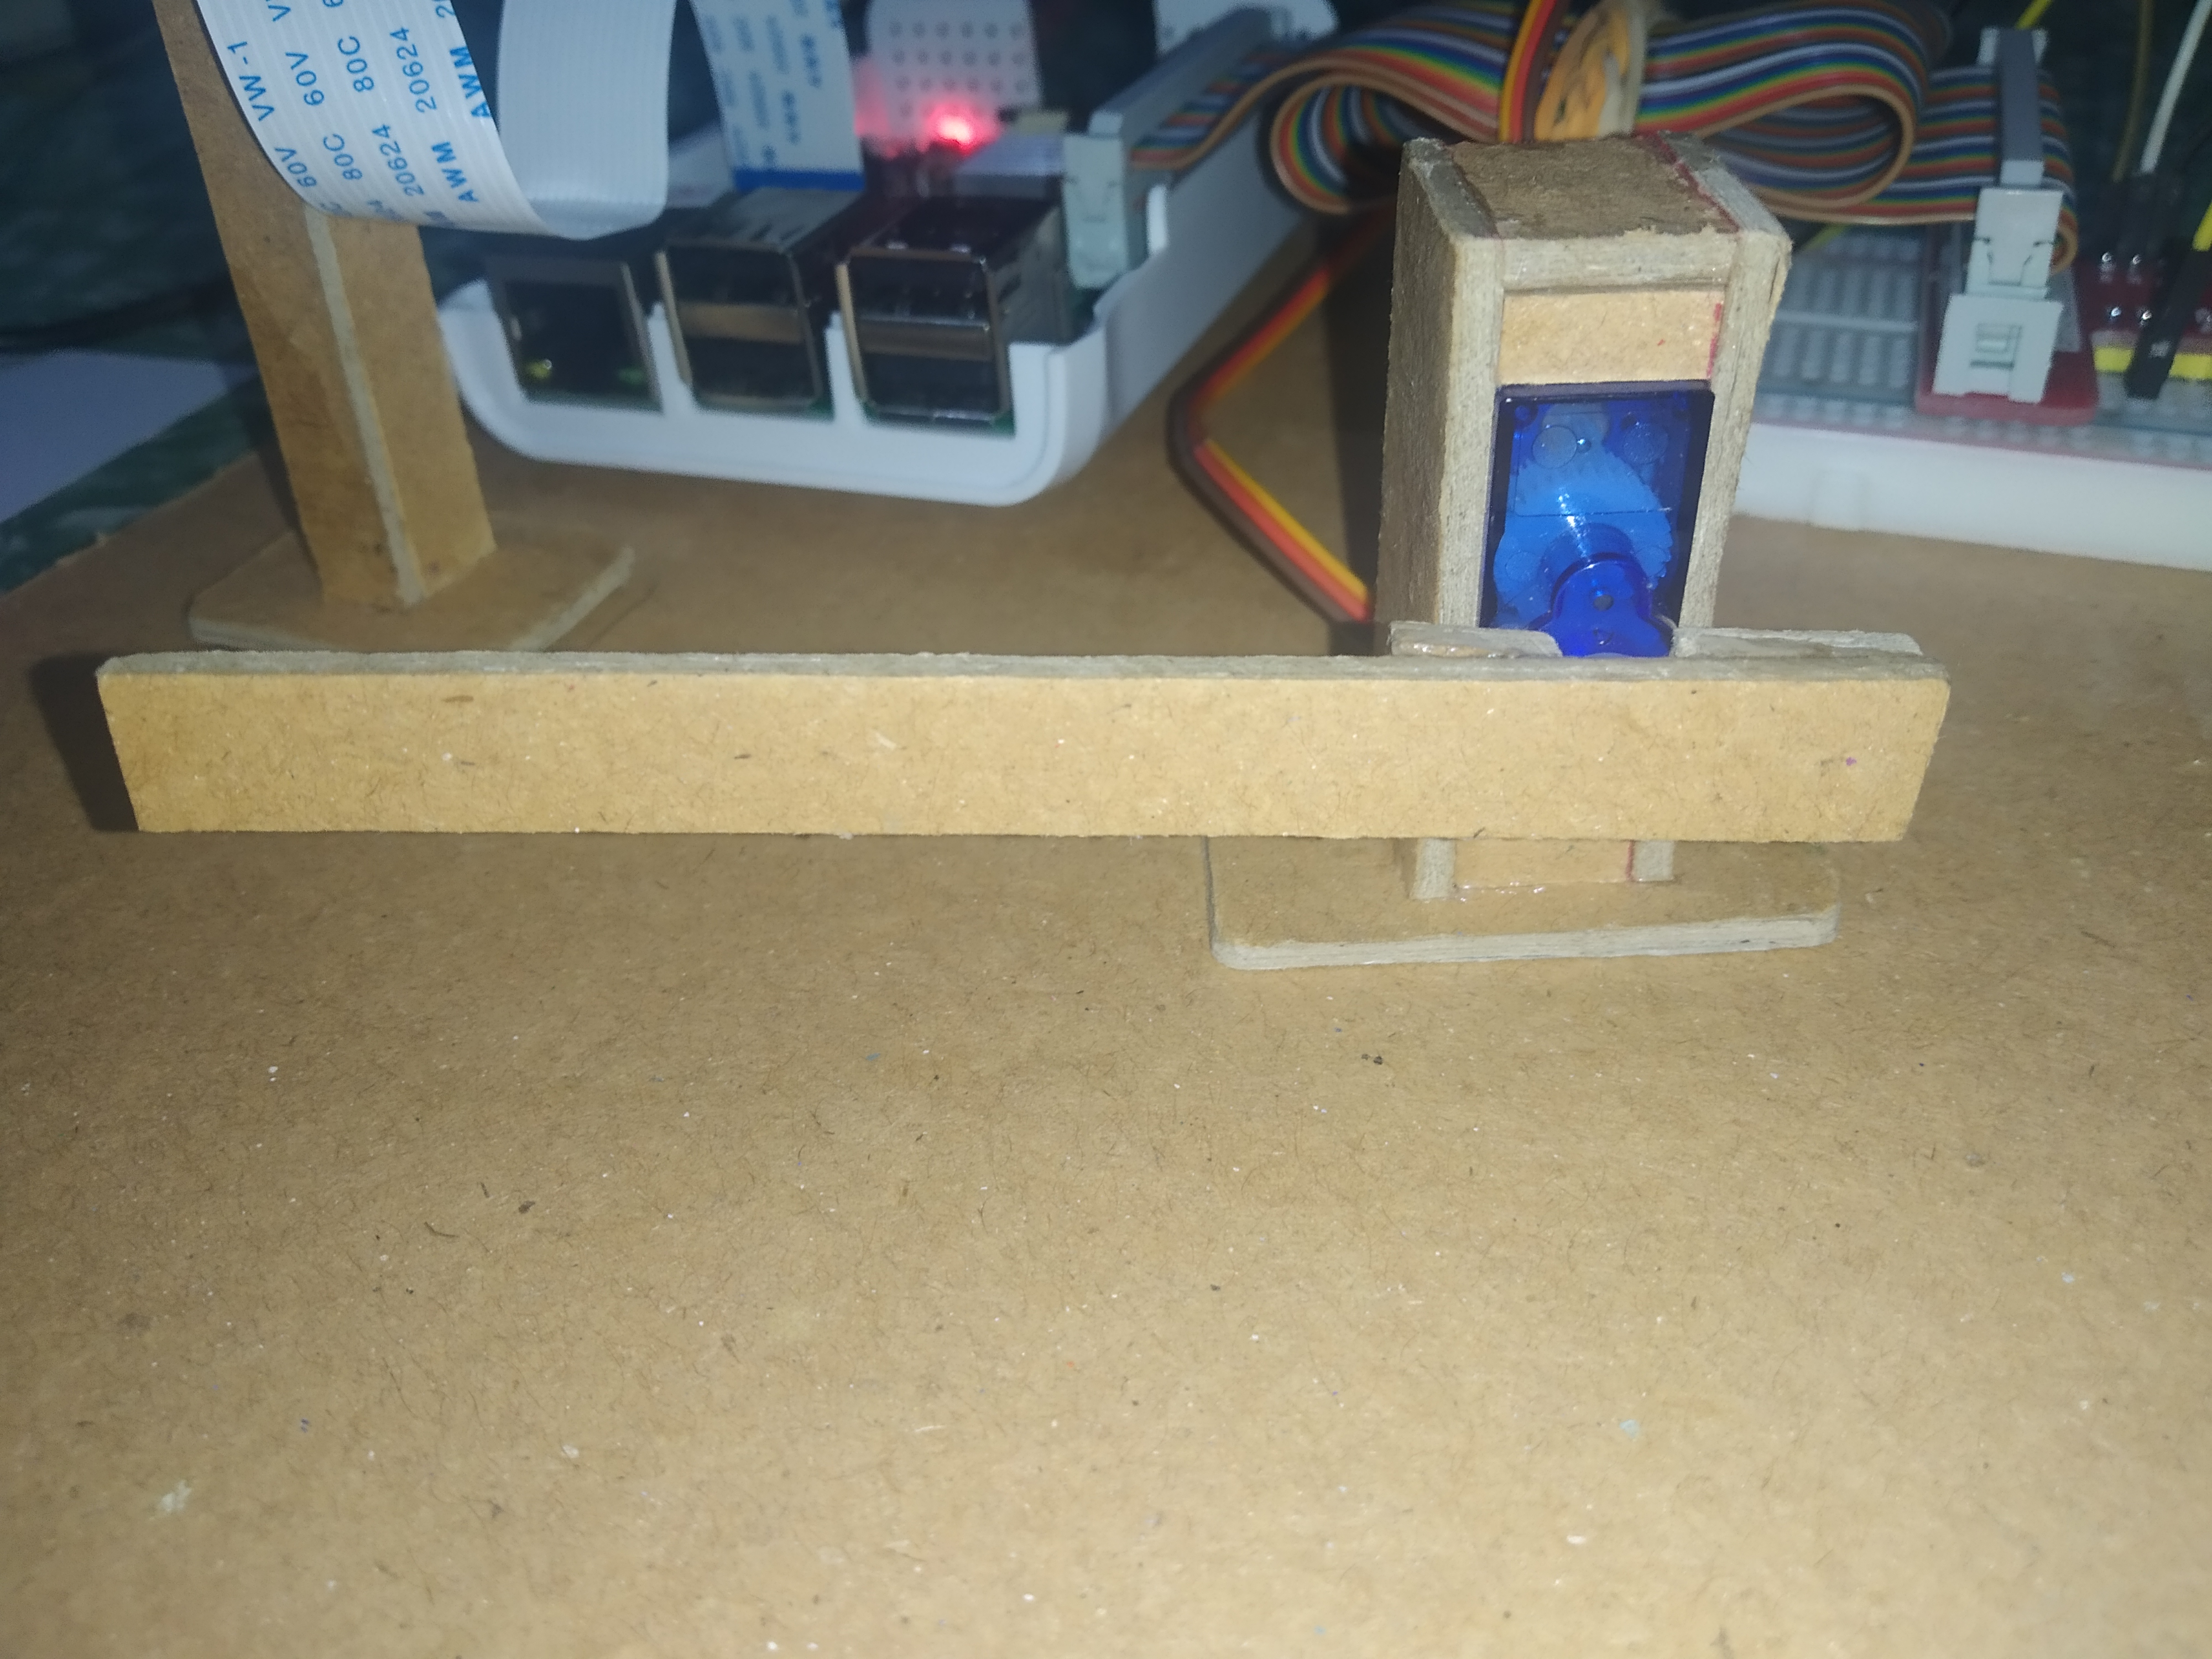
\includegraphics[height=7cm, width=0.5\textwidth, center]{images/alat-servo.jpg}
    \caption{Hasil Rancangan Servo}
    \label{fig:alatservo}
\end{figure}

\begin{figure} [H]
    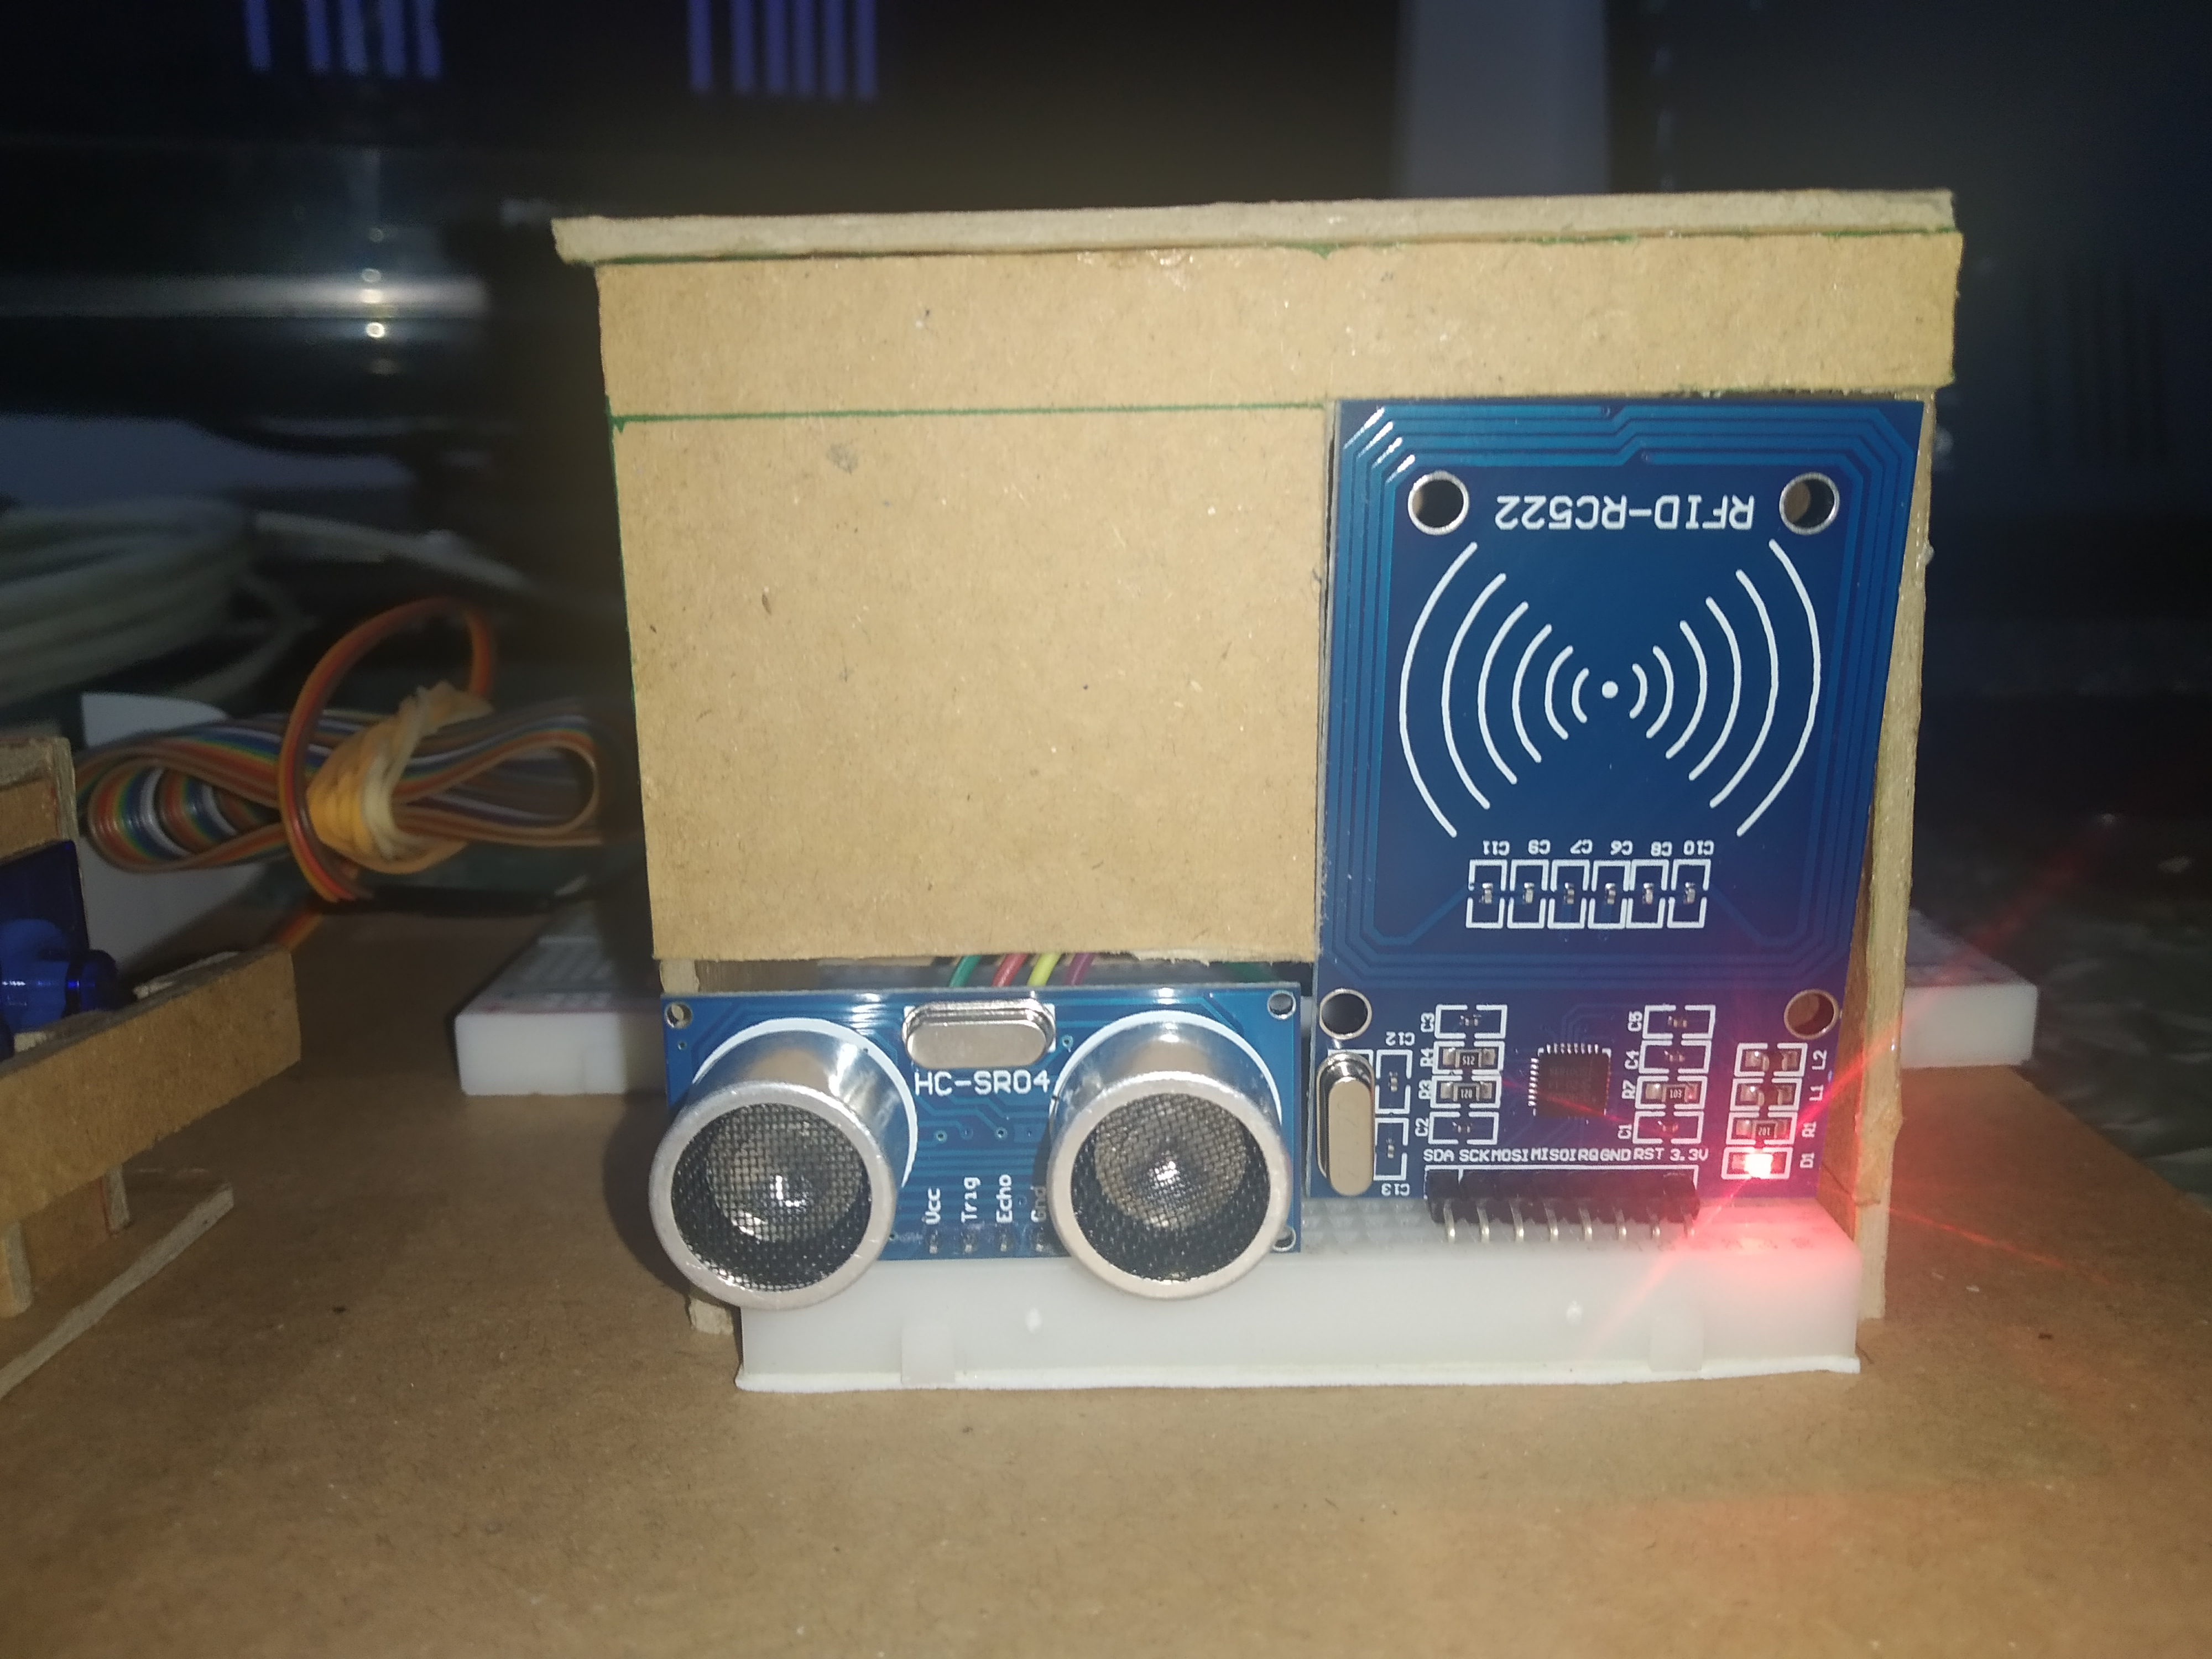
\includegraphics[height=7cm, width=0.5\textwidth, center]{images/alat-ultra&rfid.jpg}
    \caption{Hasil Rancangan Ultrasonik dan RFID}
    \label{fig:alatultrarfid}
\end{figure}

\begin{figure} [H]
    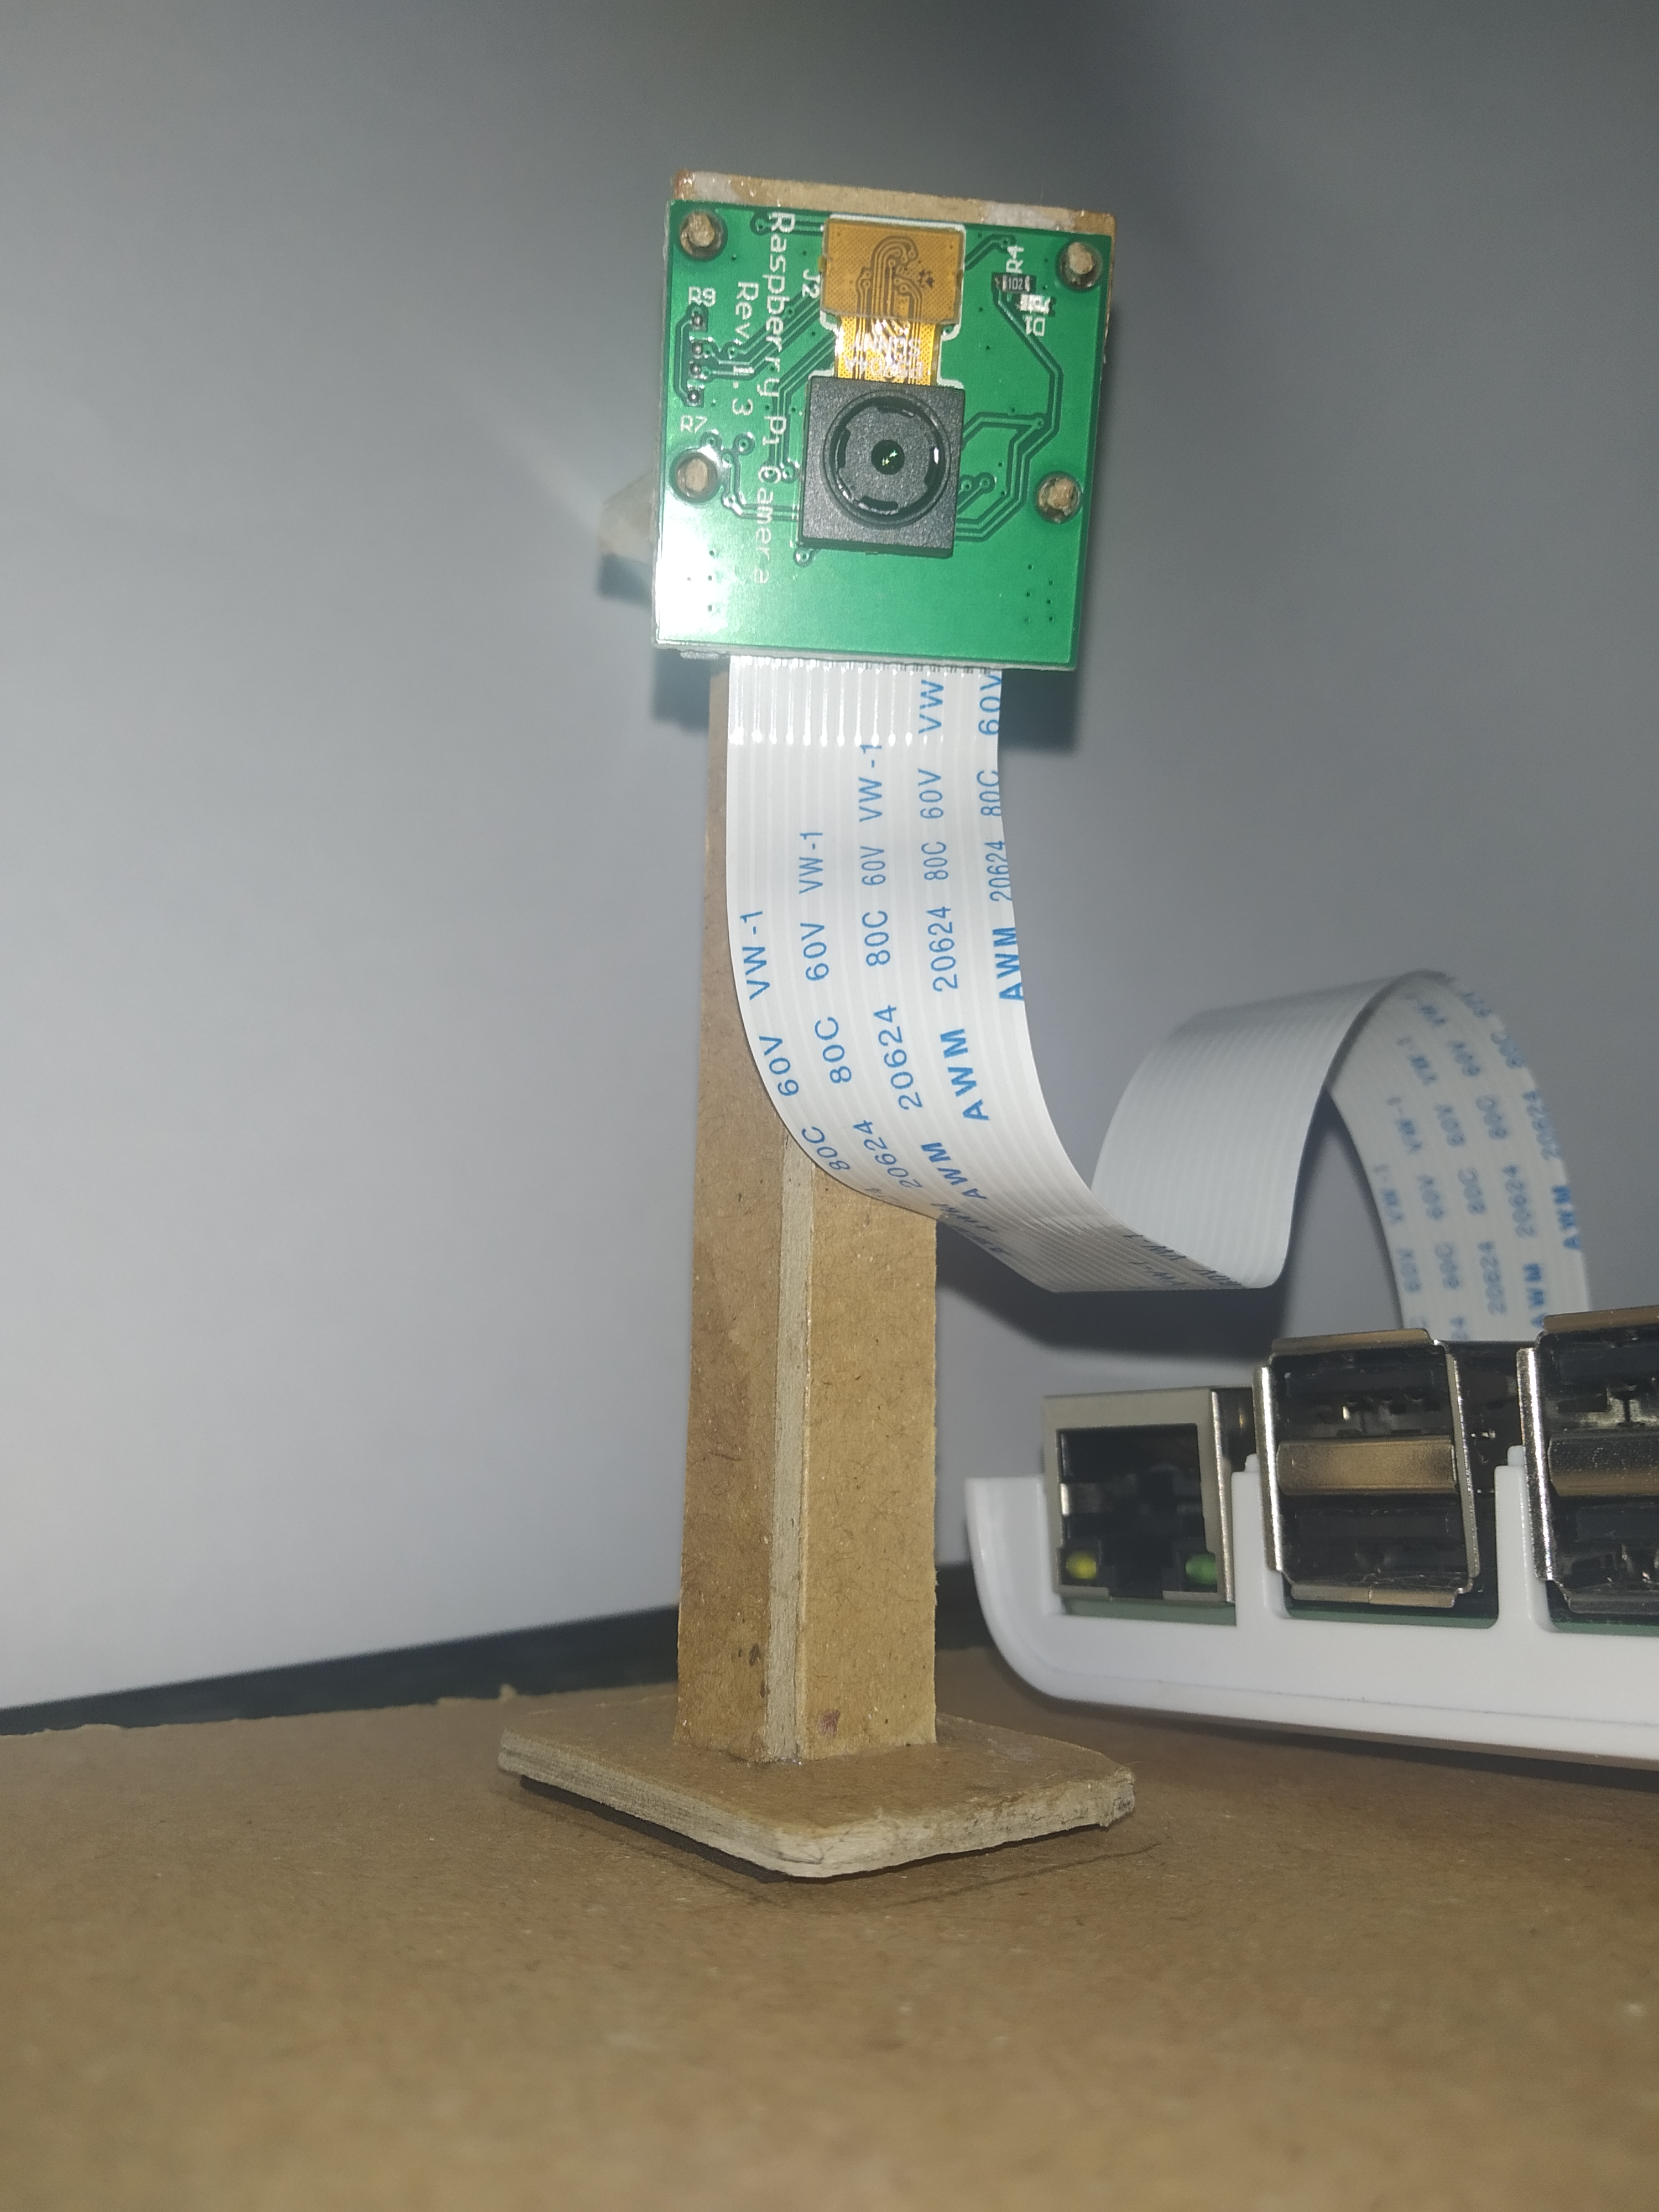
\includegraphics[height=7cm, width=0.5\textwidth, center]{images/alat-kamera.jpg}
    \caption{Hasil Rancangan Kamera}
    \label{fig:alatkamera}
\end{figure}

Pada gambar diatas merupakan rangkaian perangkat keras untuk penelitian di mana seluruh perangkat dirangkai menjadi satu rangkaian.  Gambar ~\ref{fig:alatfullmobil} merupakan hasil dari rancangan dari penelitian yang dilakukan, yang dimana masih bersifat \textit{prototype}. Pada gambar ~\ref{fig:alatservo} dapat dilihat bahwa servo digambarkan sebagai palang parkir. Pada gambar ~\ref{fig:alatultrarfid} dapat dilihat sensor ultrasonik yang akan membaca jarak dari kendaraan untuk menentukan apakah kendaraan masih ada atau sudah tidak ada dan sensor rfid untuk membaca kartu atau tag dari pengendara. Pada gambar ~\ref{fig:alatkamera} dapat dilihat kamera raspberry yang digunakan untuk mengambil nomor plat kendaraan.

\subsection{Raspberry Pi dan RFID MFRC522}
\begin{figure} [H]
    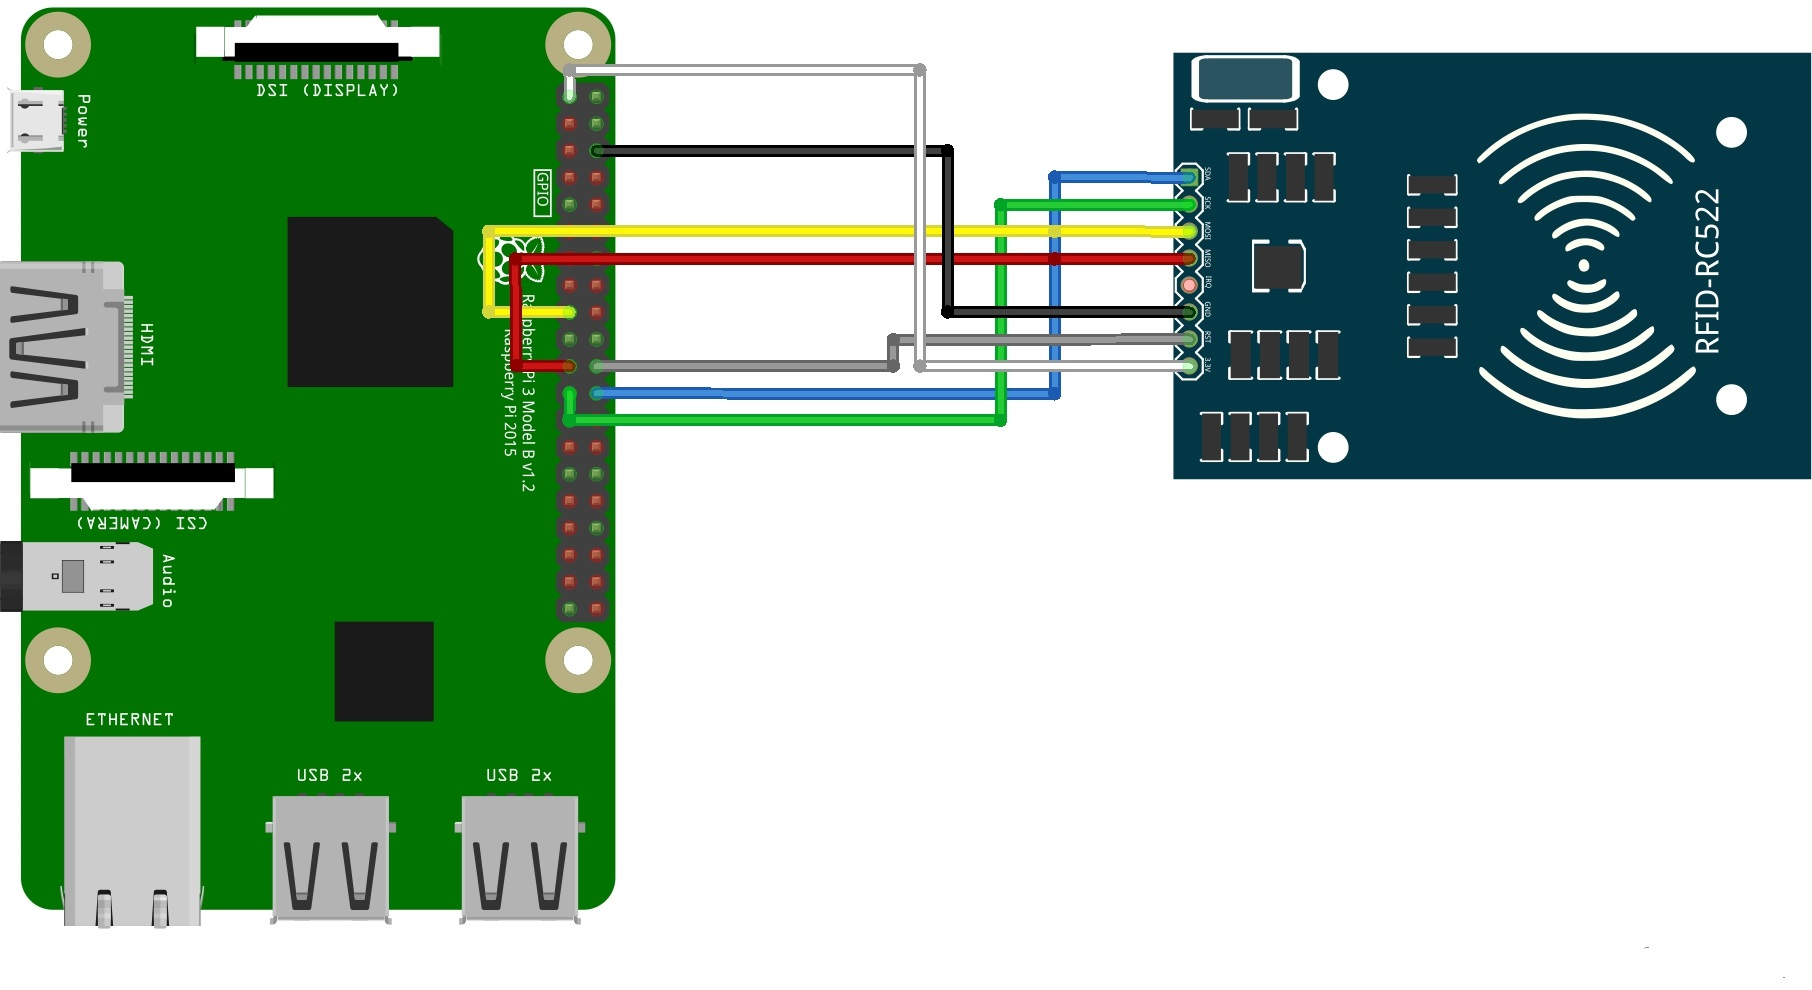
\includegraphics[width=0.85\textwidth, center]{images/skematik_rfid.jpg}
    \caption{Ragkaian Raspberry Pi dan RFID}
    \label{fig:skematikRfid}
\end{figure}

Berdasarkan gambar ~\ref{fig:skematikRfid} Menunjukkan Raspberry Pi sebagai mikrokontroler untuk menghubungkan sensor RFID yang akan membaca kartu atau tag dari pengendara. Untuk pin pada Raspberry Pi dihubungkan pada sensor RFID dapat dilihat pada tabel ~\ref{table:tableRfid}.

\begin{atable}
    \caption{Rangkaian pin RFID ke Raspberry Pi}
    \label{table:tableRfid}
    \csvreader[
        % column count = 11,
        tabular=cc,
        head to column names,
        before table=\rowcolors{2}{gray!15}{gray!30},
        table head= \rowcolor{gray!50!black} 
            \color{white} RFID & 
            \color{white} RASPBERRY PI 
            \\]
        {tables/tablerfid.csv}
        {
            RFID=\RFID, 
            RASPBERRYPI=\RASPBERRYPI}
        {
            \RFID & 
            \RASPBERRYPI}
\end{atable}

\subsection{Raspberry Pi dan HC-SR04}
\begin{figure} [H]
    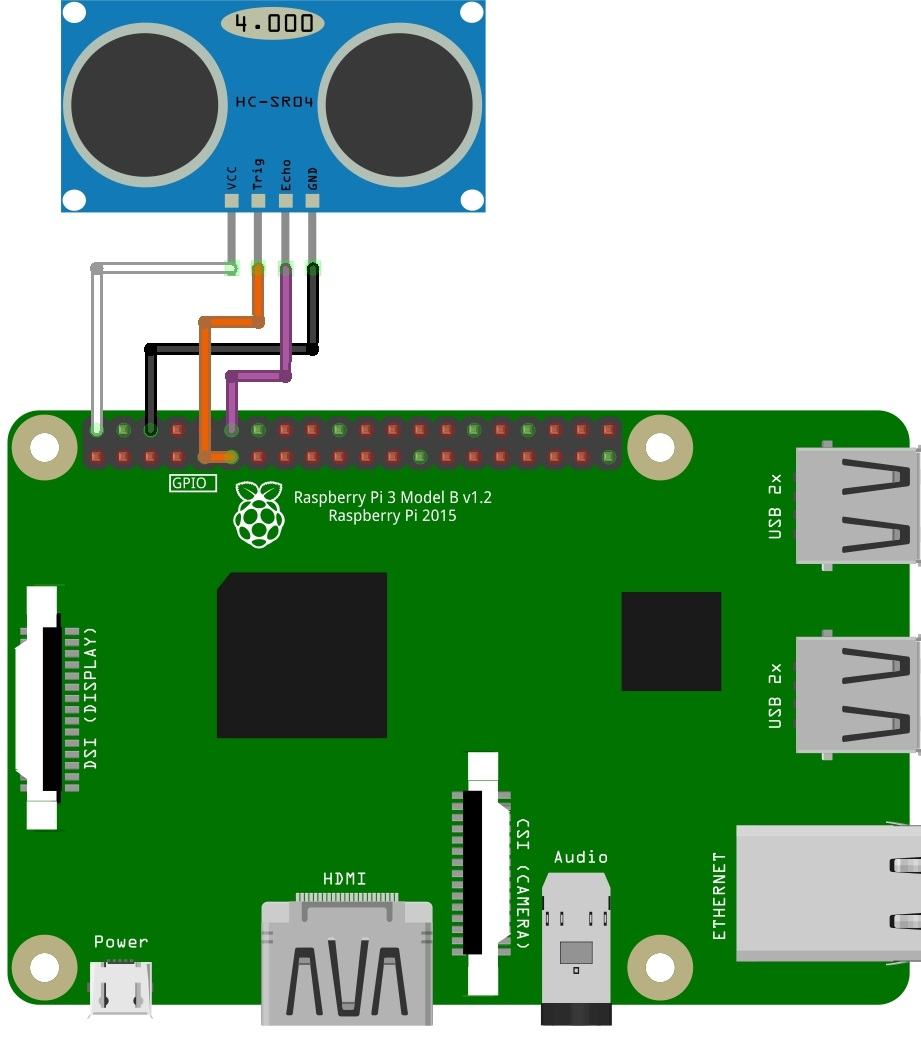
\includegraphics[height=7cm, width=0.5\textwidth, center]{images/skematik_ultra.jpg}
    \caption{Ragkaian Raspberry Pi dan Ultrasonik}
    \label{fig:skematikUltrasonik}
\end{figure}

Gambar ~\ref{fig:skematikUltrasonik} merupakan gambar rangkaian Raspberry Pi dan sensor ultrasonik. Sensor ultrasonik berfungsi sebagai indikator untuk menutup palang parkir. Apabila didepan sensor ultrasonik masih ada kendaraan, maka palang parkir masih akan terbuka, sebaliknya apabila didepan sensor sudah tidak ada kendaraan, maka palang parkir akan menutup. Sensor ultrasonik yang digunakan adalah HC-SR04 yang mempunyai 4 pin yaitu pin \textit{ground} (-), pin \textit{echo}, pin \textit{trigger}, dan pin vcc (+). Untuk pin pada Raspberry Pi dihubungkan pada sensor HC-SR04 dapat dilihat pada tabel ~\ref{table:tableUltrasonic}.

\begin{atable}
    \caption{Rangkaian pin Ultrasonik ke Raspberry Pi}
    \label{table:tableUltrasonic}
    \csvreader[
        % column count = 11,
        tabular=cc,
        head to column names,
        before table=\rowcolors{2}{gray!15}{gray!30},
        table head= \rowcolor{gray!50!black} 
            \color{white} ULTRASONIK & 
            \color{white} RASPBERRY PI 
            \\]
        {tables/tableultrasonic.csv}
        {
            ULTRASONIC=\ULTRASONIC, 
            RASPBERRYPI=\RASPBERRYPI}
        {
            \ULTRASONIC & 
            \RASPBERRYPI}
\end{atable}

\subsection{Raspberry Pi dan SG90}
\begin{figure} [H]
    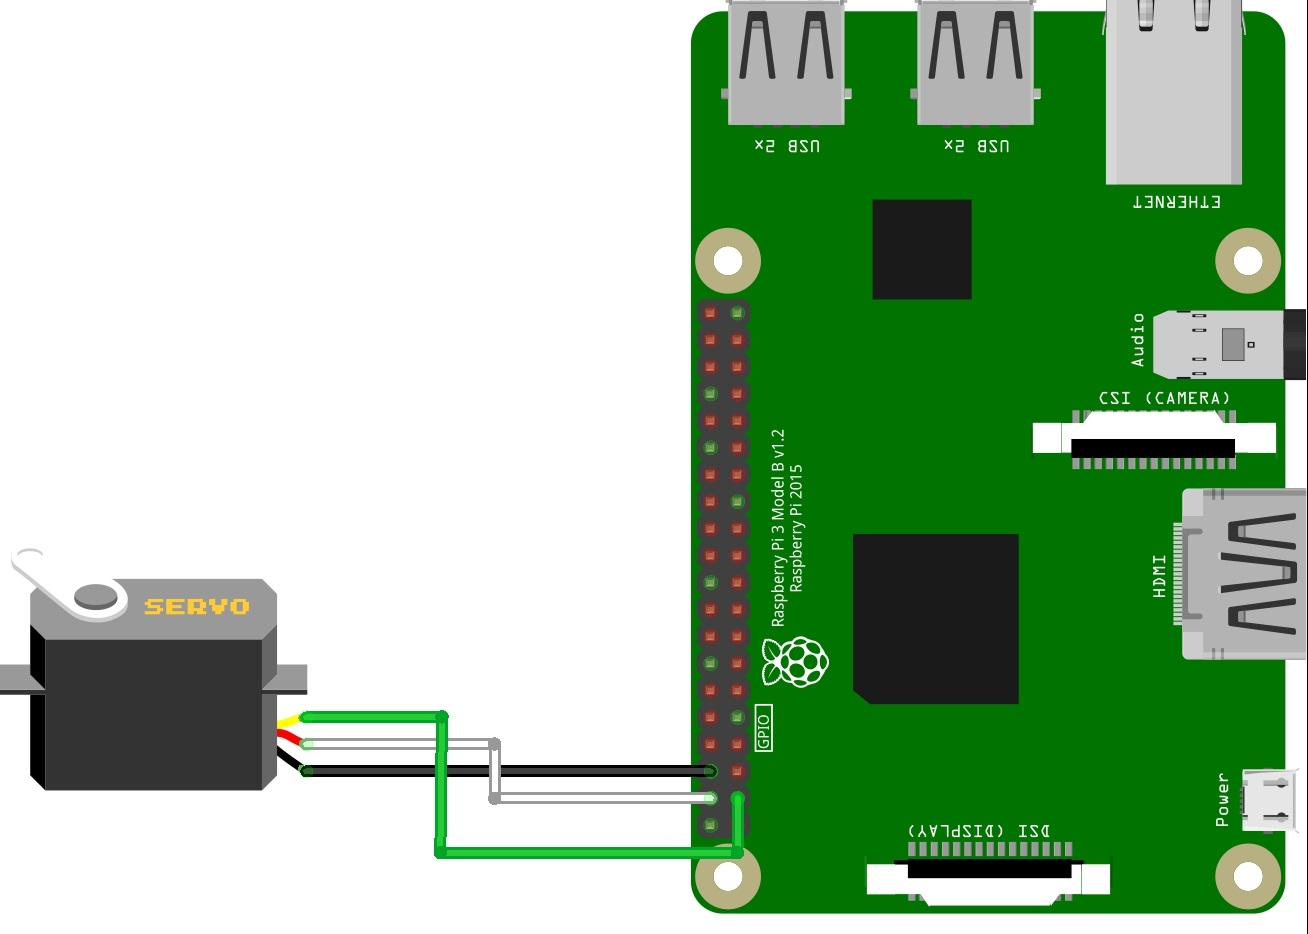
\includegraphics[height=7cm, width=0.6\textwidth, center]{images/skematik_servo.jpg}
    \caption{Ragkaian Raspberry Pi dan Servo}
    \label{fig:skematikServo}
\end{figure}

Pada penelitian ini yang akan berfungsi sebagai palang parkir adalah servo SG90. Servo yang digunakan mempunyai 3 pin yaitu pin \textit{ground} (-), pin pwm, dan pin 5v (+). Untuk pin pada Raspberry Pi dihubungkan pada servo SG90 dapat dilihat pada tabel ~\ref{table:tableServo}.

\begin{atable}
    \caption{Rangkaian pin Servo ke Raspberry Pi}
    \label{table:tableServo}
    \csvreader[
        % column count = 11,
        tabular=cc,
        head to column names,
        before table=\rowcolors{2}{gray!15}{gray!30},
        table head= \rowcolor{gray!50!black} 
            \color{white} SERVO & 
            \color{white} RASPBERRY PI 
            \\]
        {tables/tableservo.csv}
        {
            SERVO=\SERVO, 
            RASPBERRYPI=\RASPBERRYPI}
        {
            \SERVO & 
            \RASPBERRYPI}
\end{atable}

\subsection{Raspberry Pi dan Kamera Pi}
\begin{figure} [H]
    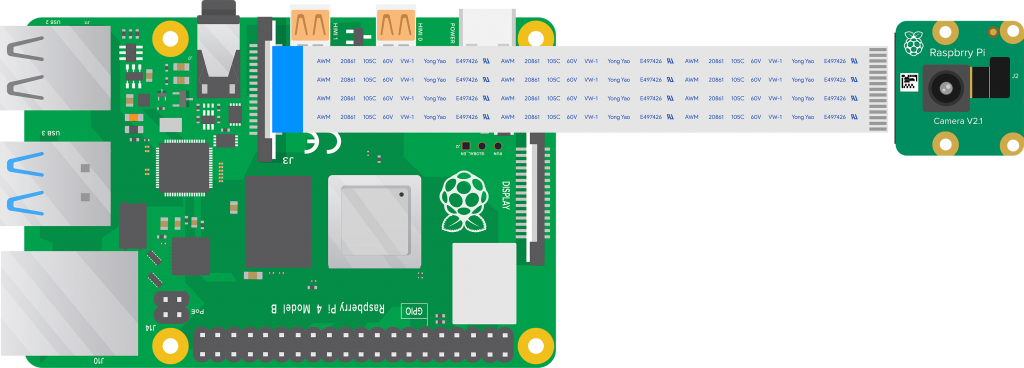
\includegraphics[width=0.85\textwidth, center]{images/skematik-kamera.png}
    \caption{Ragkaian Raspberry Pi dan Kamera}
    \label{fig:skematikKamera}
\end{figure}

Gambar ~\ref{fig:skematikKamera} merupakan gambar skematik Raspberry Pi dengan Kamera. Untuk menghubungkan Raspberry Pi dengan kamera cukup dengan menghubungkan kamera dengan port \textit{Camera Serial Interface} (CSI) yang sudah tersedia pada Raspberry Pi.

% \subsection{Hasil Perancangan Perangkat Lunak}

\section{Hasil Rancangan Aplikasi Web}

\subsection{Activity Diagram}

\subsection{Struktur \textit{Database}}
Nama \textit{database} : skripsi

Pada \textit{database} aplikasi ini, tabel dibagi menjadi 5 tabel sebagai berikut:

\begin{enumerate}[topsep=0pt,itemsep=0pt,partopsep=0pt, parsep=0pt]
    \item Tabel rfid\_tag

    Nama Tabel : rfid\_tag

    \textit{Primary Key} : id

    \begin{atable}
        \caption{rfid\_tag}
        \label{table:db_rfid_tag}
        \csvreader[
            % column count = 11,
            tabular=cc,
            head to column names,
            before table=\rowcolors{2}{gray!15}{gray!30},
            table head= \rowcolor{gray!50!black} 
                \color{white} \textit{Coloumn} & 
                \color{white} \textit{Type} 
                \\]
            {tables/db_rfid_tag.csv}
            {
                Coloumn=\Coloumn, 
                Type=\Type}
            {
                \Coloumn & 
                \Type}
    \end{atable}

    Atribut \textit{id} pada tabel rfid\_tag berfungsi sebagai kunci utama. Atribut jenis\_kendaraan digunakan untuk menentukan jenis kendaraan yang digunakan oleh pengemudi. Atribut saldo digunakan untuk menyimpan saldo dari pengemudi.

    \item Tabel tempat\_parkir

    Nama Tabel : tempat\_parkir

    \textit{Primary Key} : id

    \begin{table} [H]
        \centering
        \caption{tempat\_parkir}
        \label{table:db_tempat_parkir}
        \csvreader[
            % column count = 11,
            tabular=cc,
            head to column names,
            before table=\rowcolors{2}{gray!15}{gray!30},
            table head= \rowcolor{gray!50!black} 
                \color{white} \textit{Coloumn} & 
                \color{white} \textit{Type} 
                \\]
            {tables/db_tempat_parkir.csv}
            {
                Coloumn=\Coloumn, 
                Type=\Type}
            {
                \Coloumn & 
                \Type}
    \end{table}

    Tabel tempat\_parkir mempunyai atribut \textit{id} yang berfungsi sebagai kunci utama, atribut \textit{id} juga berfungsi sebagai nomor slot tempat parkir. Atribut jenis digunakan untuk menentukan jenis dari slot parkir. Atribut tarif digunakan sebagai tarif per jam dari slot parkir. Atribut status digunakan untuk mengetahui apakah slot sedang tersedia atau terpakai.

    \item Tabel kendaraan

    Nama Tabel : kendaraan

    \textit{Primary Key} : id

    \textit{Foreign Key} : id\_rfid\_tag

    % \begin{table} [H]
    %     \centering 
    %     \caption{kendaraan}
    %     \label{table:db_kendaraan}
    %     \csvreader[
    %         % column count = 11,
    %         tabular=cc,
    %         head to column names,
    %         before table=\rowcolors{2}{gray!15}{gray!30},
    %         table head= \rowcolor{gray!50!black} 
    %             \color{white} \textit{Coloumn} & 
    %             \color{white} \textit{Type} 
    %             \\]
    %         {tables/db_kendaraan.csv}
    %         {
    %             Coloumn=\Coloumn, 
    %             Type=\Type}
    %         {
    %             \Coloumn & 
    %             \Type}
    % \end{table}

    Tabel kendaraan mempunyai atribut \textit{id} yang berfungsi sebagai kunci utama. Atribut nomor\_plat berfungsi untuk menyimpan nomor plat pengendara. Atribut id\_rfid\_tag didapat dari tabel rfid\_tag.

    \item Tabel parkir

    Nama Tabel : parkir

    \textit{Primary Key} : id

    \textit{Foreign Key} : id\_rfid\_tag, id\_tempat\_parkir

    % \begin{table} [H]
    %     \centering
    %     \caption{parkir}
    %     \label{table:db_parkir}
    %     \csvreader[
    %         % column count = 11,
    %         tabular=cc,
    %         head to column names,
    %         before table=\rowcolors{2}{gray!15}{gray!30},
    %         table head= \rowcolor{gray!50!black} 
    %             \color{white} \textit{Coloumn} & 
    %             \color{white} \textit{Type} 
    %             \\]
    %         {tables/db_parkir.csv}
    %         {
    %             Coloumn=\Coloumn, 
    %             Type=\Type}
    %         {
    %             \Coloumn & 
    %             \Type}
    % \end{table}

    Tabel kendaraan mempunyai atribut \textit{id} yang berfungsi sebagai kunci utama. Atribut id\_rfid\_tag didapat dari tabel rfid\_tag. Atribut nomor\_plat digunakan untuk menyimpan nomor plat pengendara. Atribut id\_tempat\_parkir didapat dari tabel tempat\_parkir. Atribut waktu\_masuk digunakan untuk mencatat waktu masuk pengendara. Atribut waktu\_keluar digunakan untuk mencatat waktu keluar pengguna.

    \item Tabel \textit{reload\_id}

    Nama Tabel : reload\_id

    \textit{Primary Key} : id

    \begin{table} [H]
        \centering
        \caption{reload\_id}
        \label{table:db_reload_id}
        \csvreader[
            % column count = 11,
            tabular=cc,
            head to column names,
            before table=\rowcolors{2}{gray!15}{gray!30},
            table head= \rowcolor{gray!50!black} 
                \color{white} \textit{Coloumn} & 
                \color{white} \textit{Type} 
                \\]
            {tables/db_reload_id.csv}
            {
                Coloumn=\Coloumn, 
                Type=\Type}
            {
                \Coloumn & 
                \Type}
    \end{table}

    Tabel reload\_id mempunyai atribut \textit{id} yang berfungsi sebagai kunci utama. Atribut uid digunakan untuk menyimpan id rfid tag.

\end{enumerate}

\subsection{Tampilan Website}
\begin{figure} [H]
    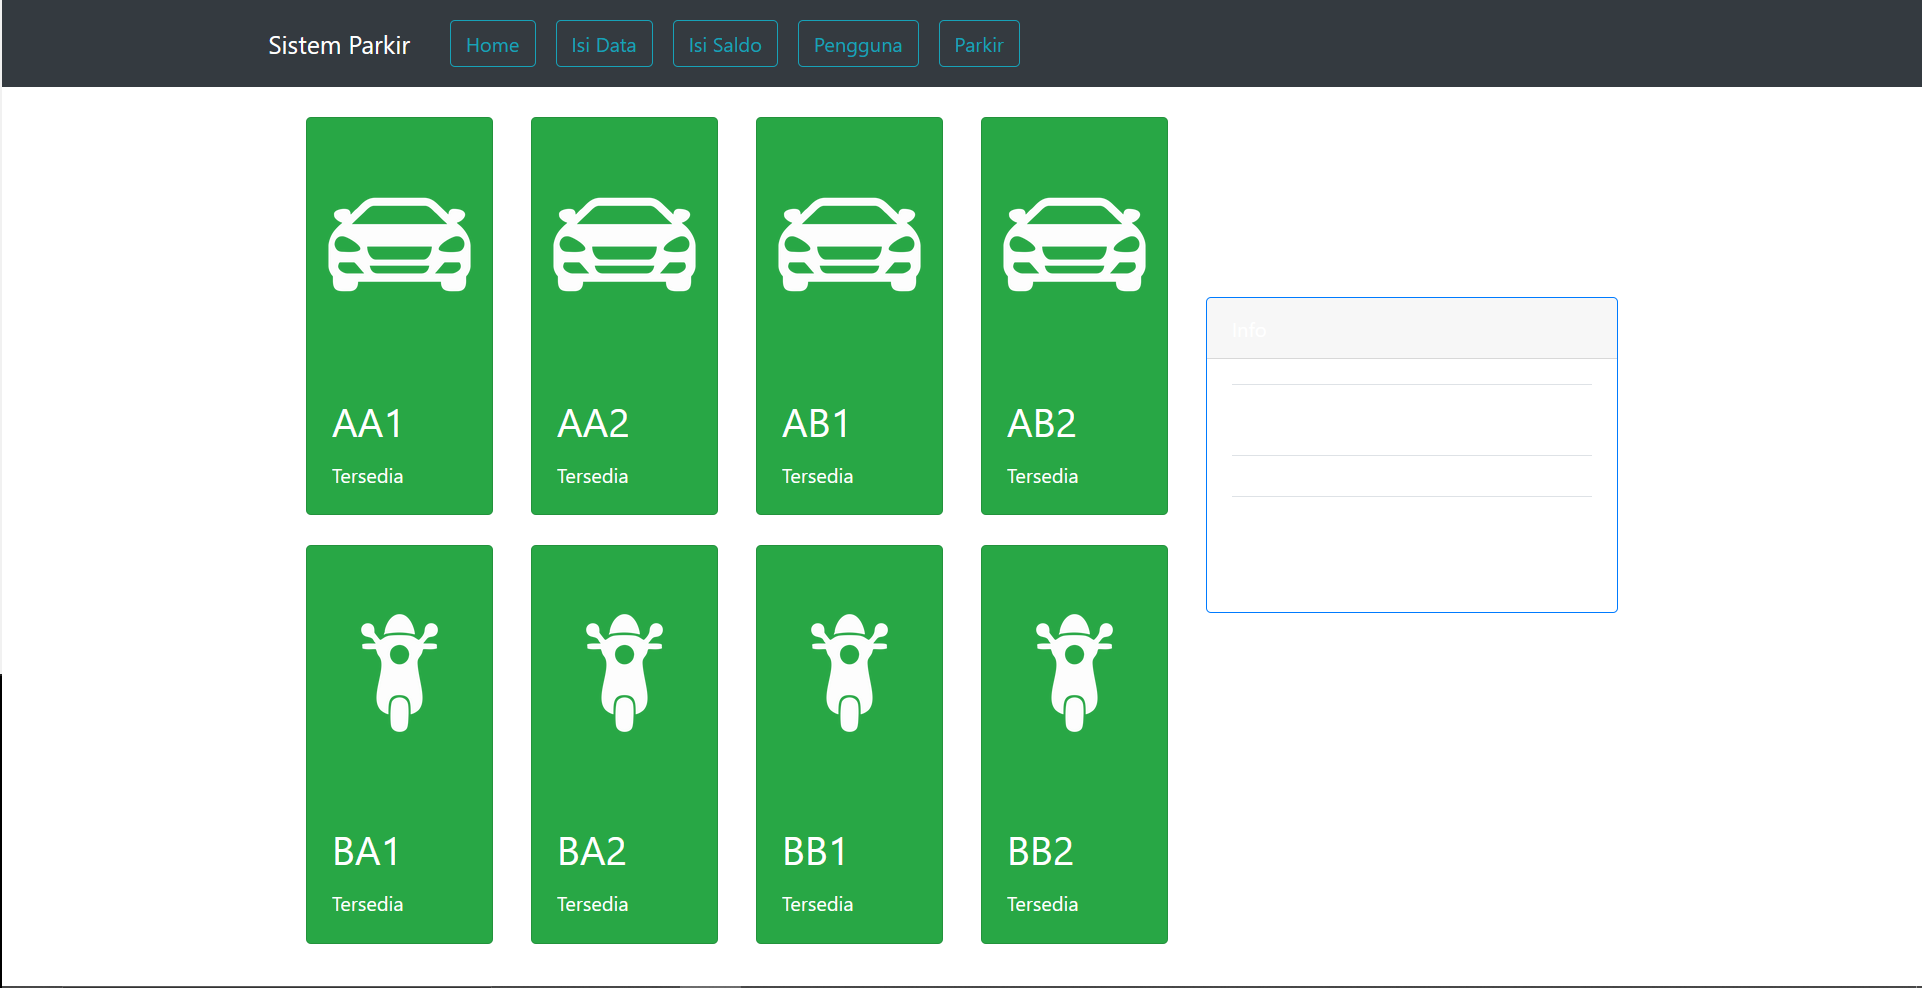
\includegraphics[width=0.85\textwidth, center]{images/web 1 layout parkir.png}
    \caption{Hasil Rancangan Kamera}
    \label{fig:web1layout-parkir}
\end{figure}

\begin{figure} [H]
    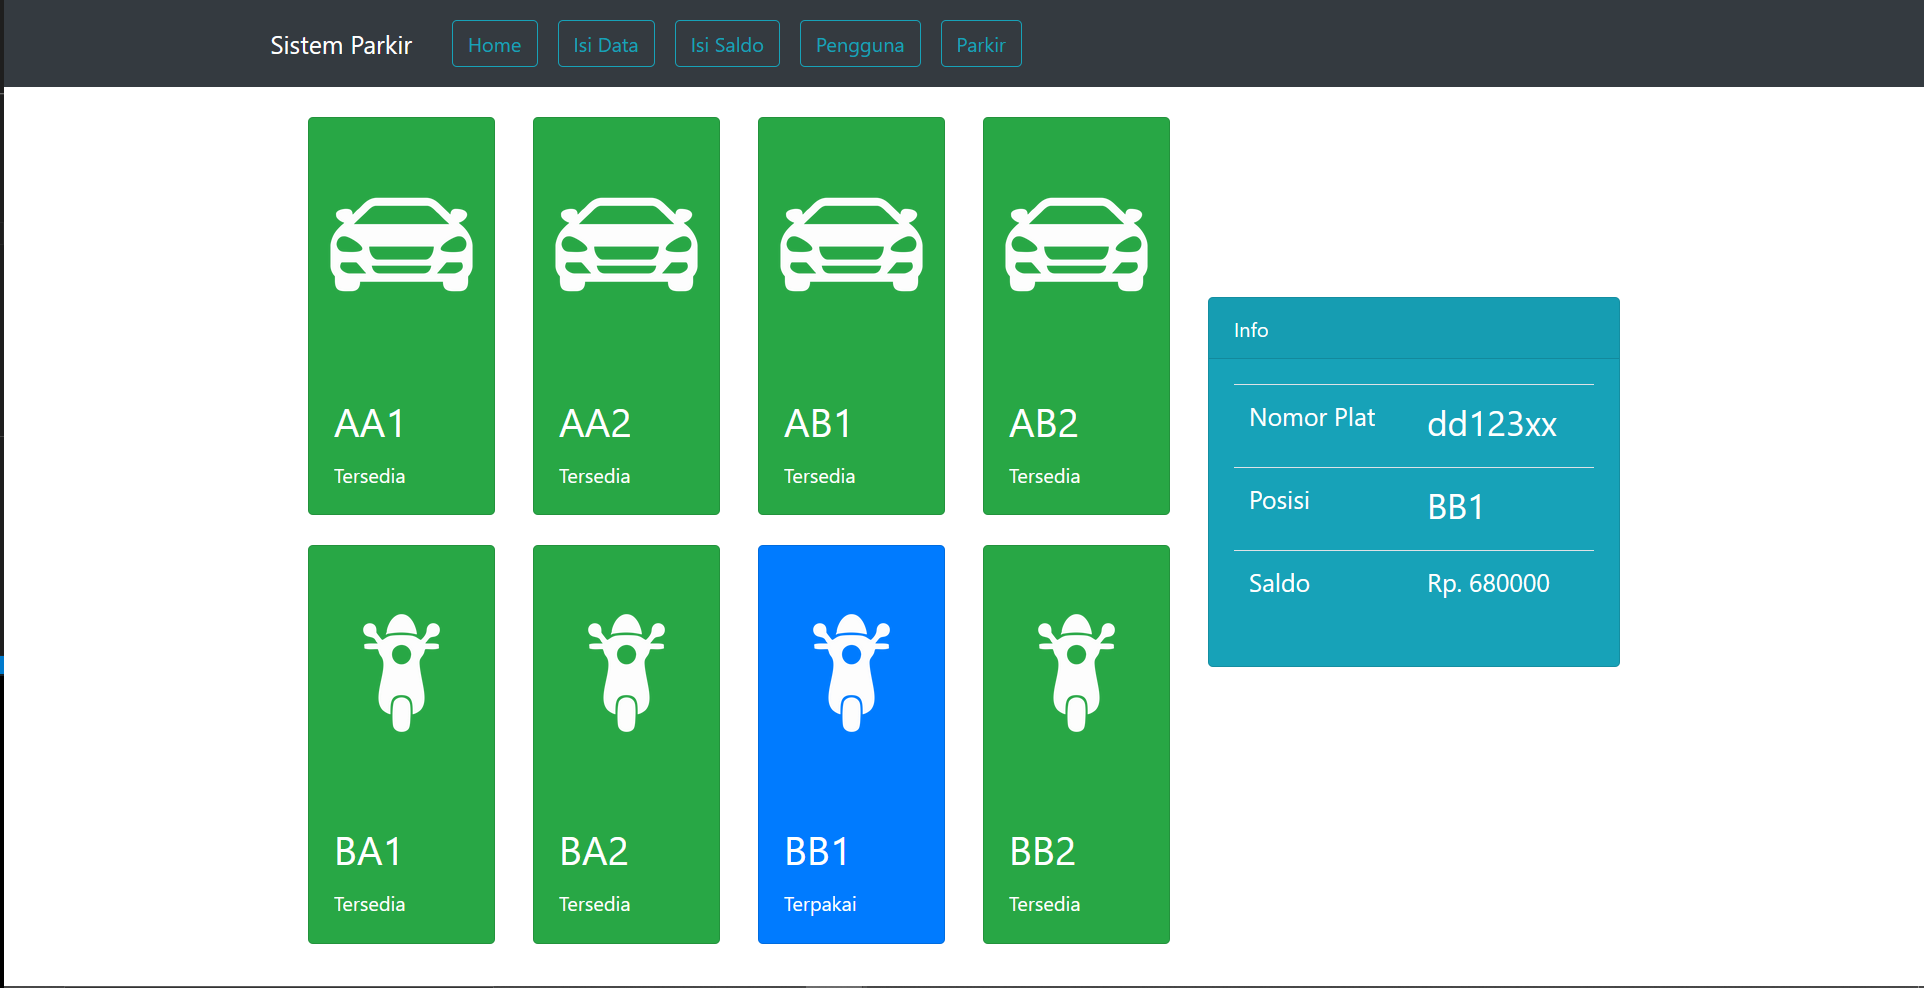
\includegraphics[width=0.85\textwidth, center]{images/web 1 layout parkir baru masuk.png}
    \caption{Hasil Rancangan Kamera}
    \label{fig:web1layout-parkir-baru-masuk}
\end{figure}

\begin{figure} [H]
    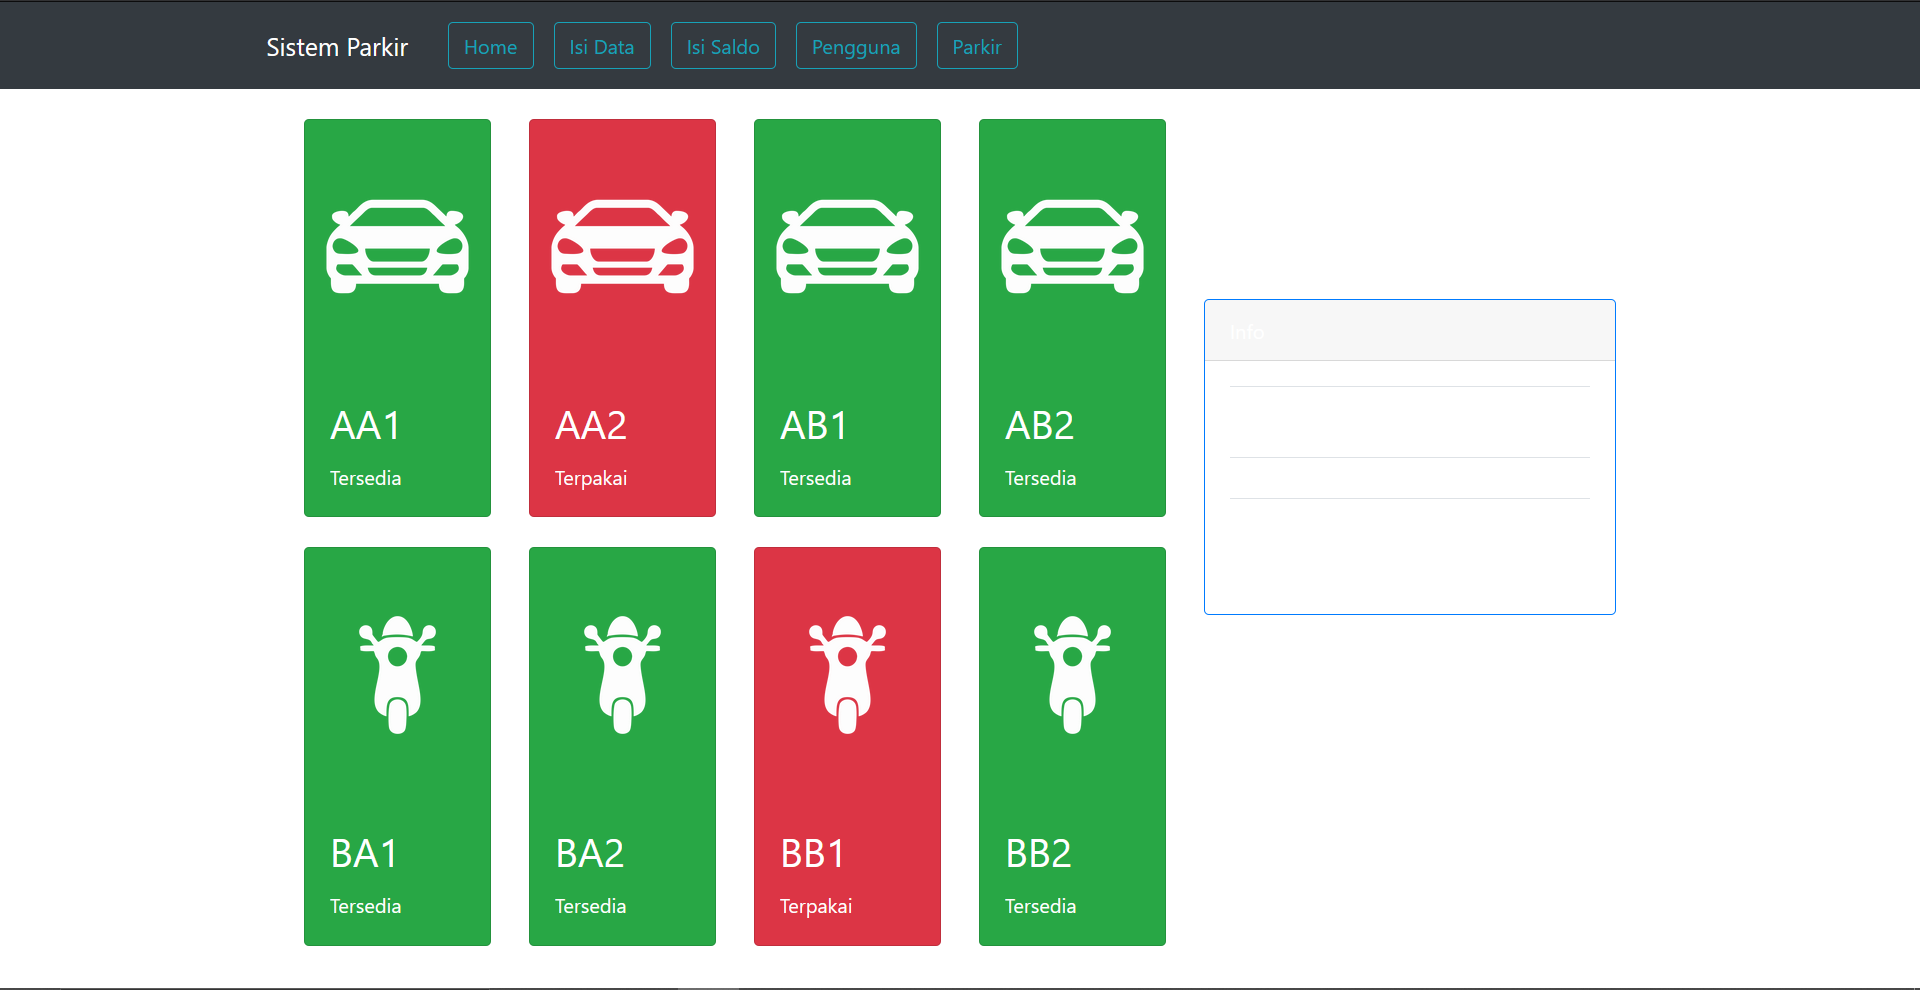
\includegraphics[width=0.85\textwidth, center]{images/web 1 layout parkir ada kendaraan.png}
    \caption{Hasil Rancangan Kamera}
    \label{fig:web1layout-parkir-ada-kendaraan}
\end{figure}

\begin{figure} [H]
    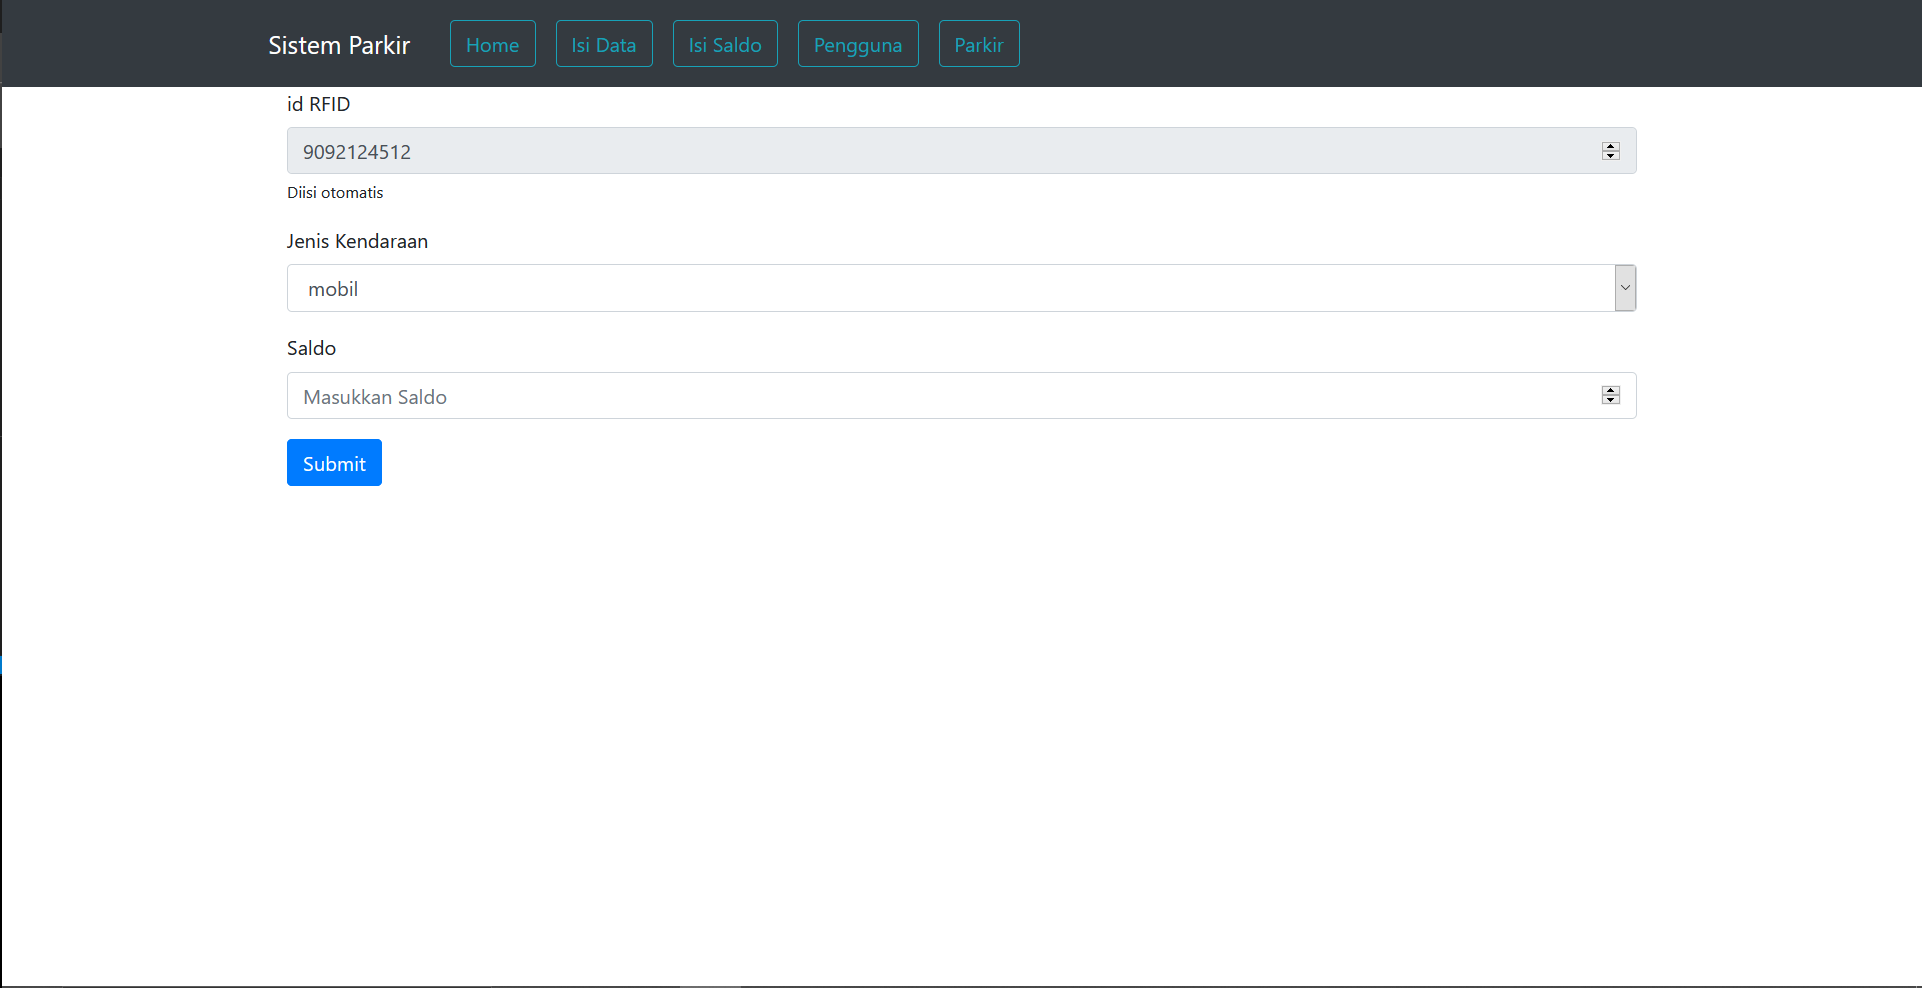
\includegraphics[width=0.85\textwidth, center]{images/web 2 isi data.png}
    \caption{Hasil Rancangan Kamera}
    \label{fig:web2isi-data}
\end{figure}

\begin{figure} [H]
    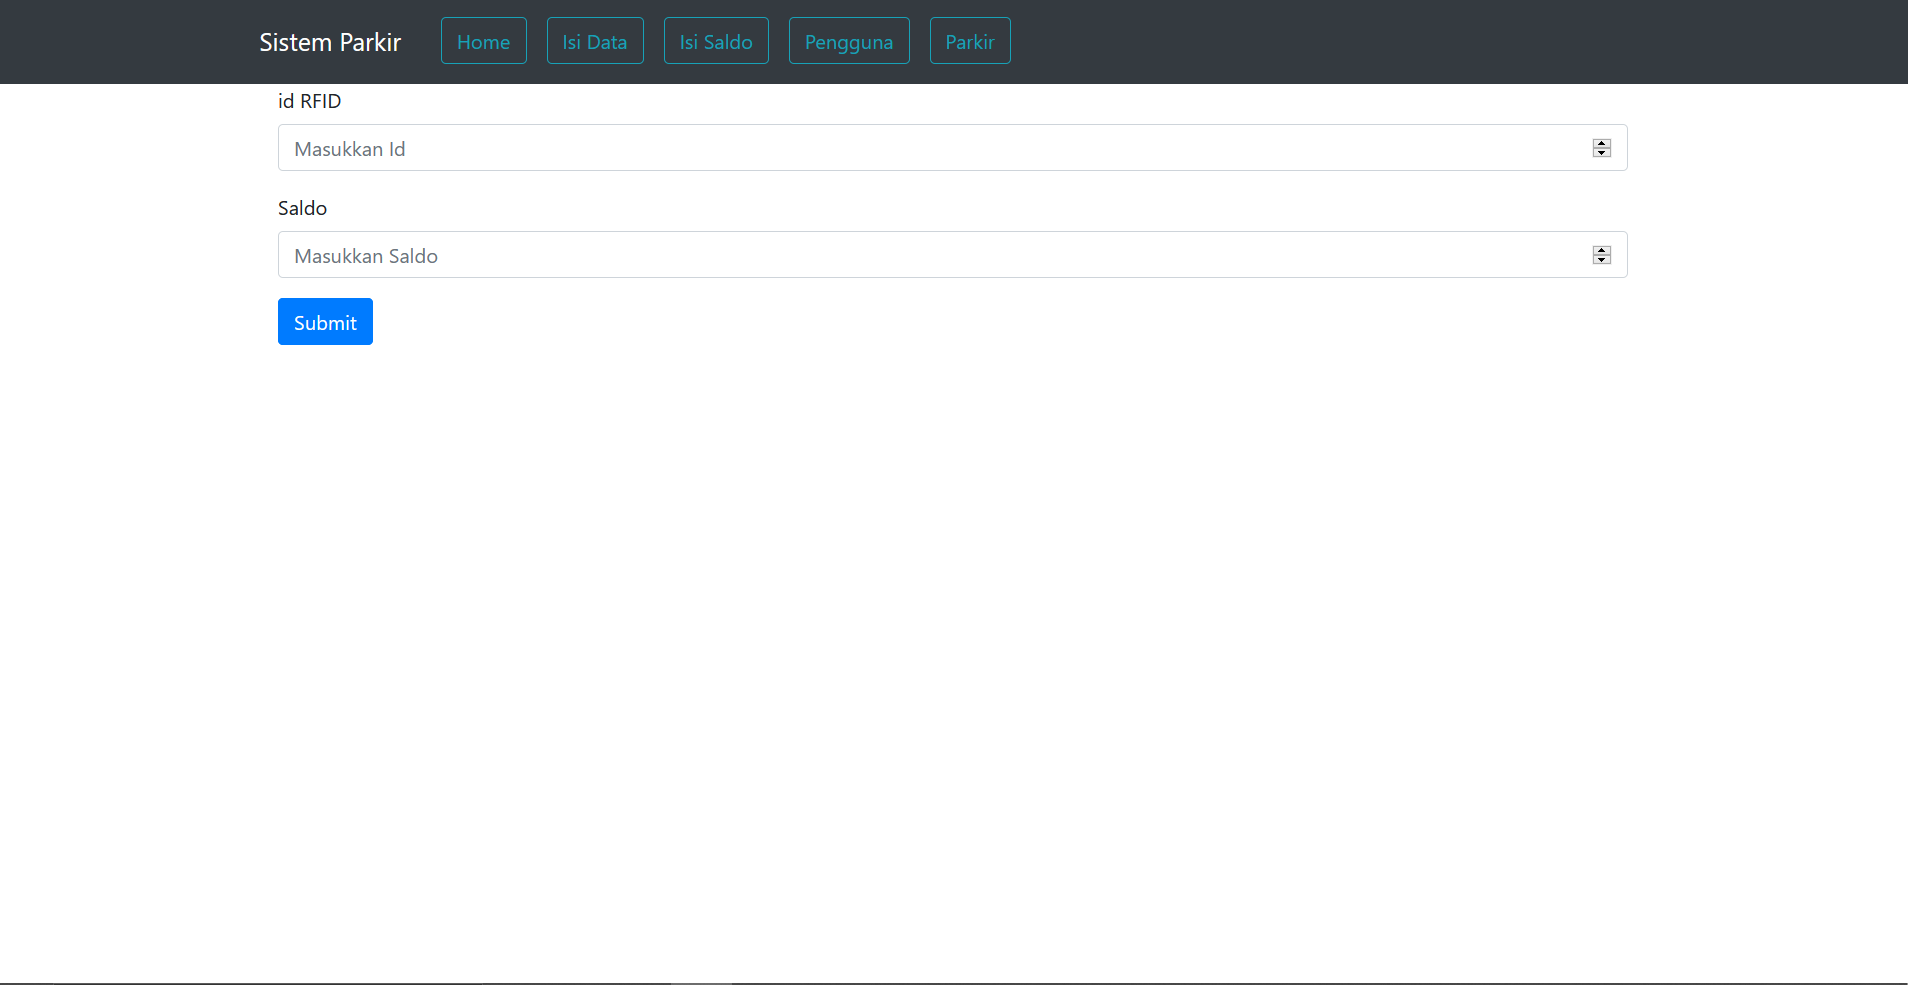
\includegraphics[width=0.85\textwidth, center]{images/web 3 isi saldo.png}
    \caption{Hasil Rancangan Kamera}
    \label{fig:web3isi-saldo}
\end{figure}

\begin{figure} [H]
    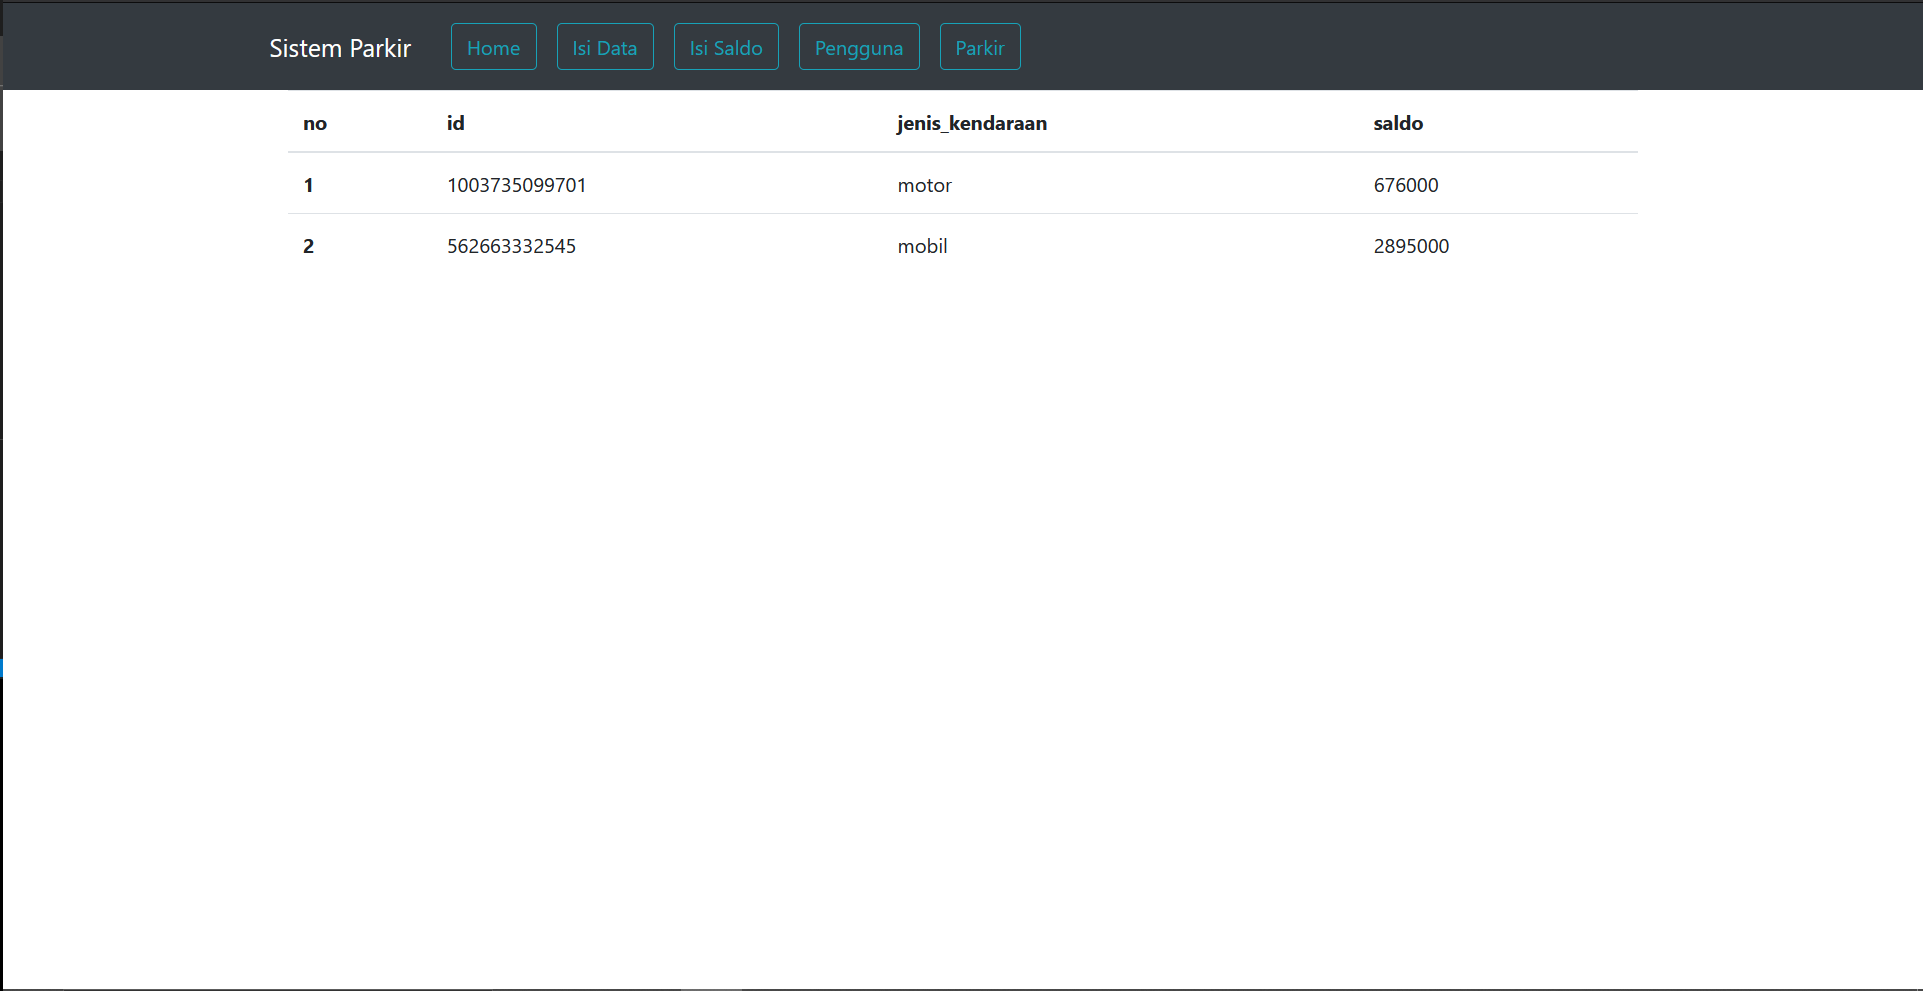
\includegraphics[width=0.85\textwidth, center]{images/web 4 pengguna.png}
    \caption{Hasil Rancangan Kamera}
    \label{fig:web4pengguna}
\end{figure}

\begin{figure} [H]
    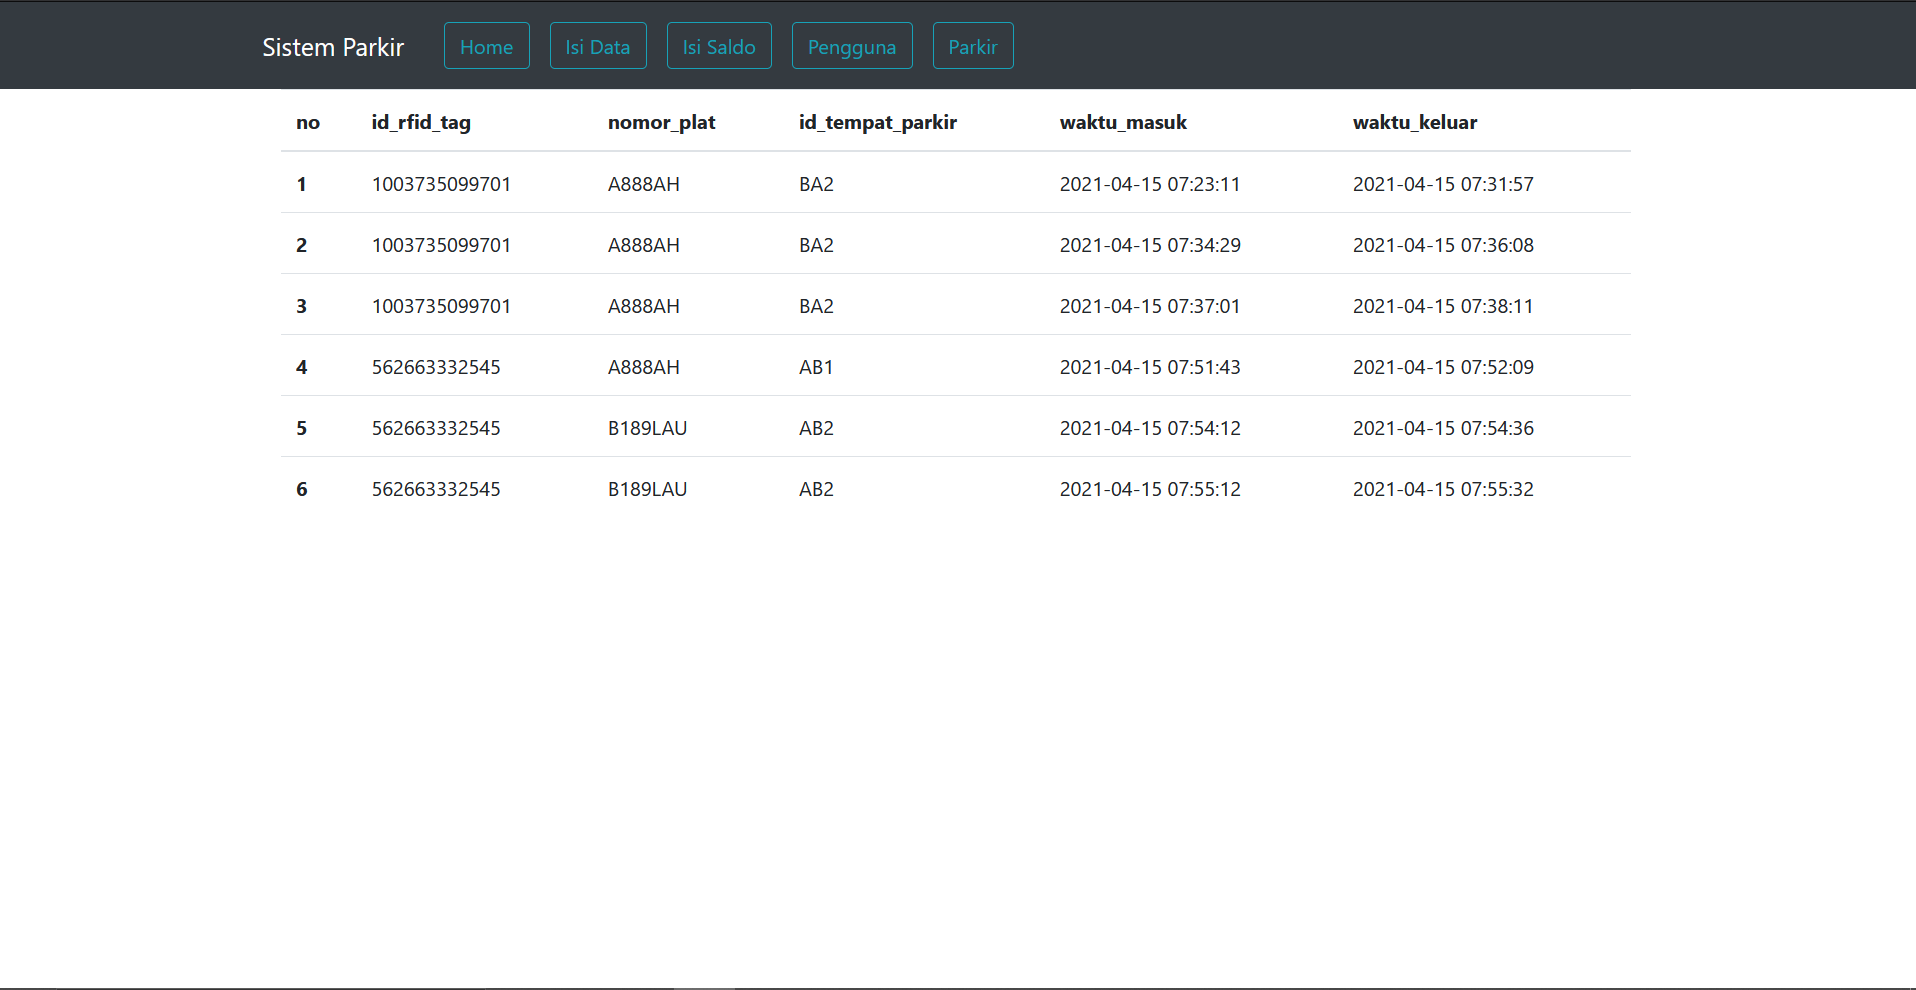
\includegraphics[width=0.85\textwidth, center]{images/web 5 informasi.png}
    \caption{Hasil Rancangan Kamera}
    \label{fig:web5informasi}
\end{figure}